\documentclass[english, version-2020-11]{uzl-thesis}
\UzLStyle{pagella contrast design}
\usepackage{comment}
\usepackage{fontspec}
\usepackage{float}
\lstset{basicstyle=\ttfamily}
\usepackage{tikz}
\usetikzlibrary{matrix}
\usepackage{pgfplots}
\usetikzlibrary{pgfplots.fillbetween}
\pgfplotsset{compat=1.18}
\usepackage{pgfplotstable}
\usepackage{pgf-umlsd}
\usepgfplotslibrary{statistics}
\usetikzlibrary{patterns} 
\usepackage{subcaption}
\usepackage{booktabs}
\usepackage{siunitx}
\usepackage[flushleft]{threeparttable}
\usepackage{enumitem}
\usepackage{multirow}
\sisetup{table-format=1.3}
\usepackage{sansmath}
\sloppy
\usetikzlibrary{shapes.geometric, arrows.meta, positioning, shadows.blur}
\usetikzlibrary{positioning,backgrounds,calc,shapes, shapes,arrows.meta}
\usepackage{xcolor}
\lstset{
    basicstyle=\ttfamily\small,
    frame=single,
    columns=fullflexible,
    breaklines=true,
    backgroundcolor=\color{gray!5},
    keywordstyle=\color{blue!70!black},
    commentstyle=\color{gray!60},
    stringstyle=\color{red!70!black},
    captionpos=b,
    showstringspaces=false,
    tabsize=4
}


\tikzstyle{process} = [
    rectangle, rounded corners,
    minimum width=4.2cm,
    minimum height=1.2cm,
    text centered,
    draw=black,
    fill=blue!10,
    font=\sffamily\small,
    blur shadow
]

\tikzstyle{arrow} = [
    thick,
    ->,
    >=Stealth,
    draw=gray!80
]

\tikzstyle{cell} = [rectangle, draw=black, minimum width=2.5em, minimum height=2.5em, anchor=center]
\tikzstyle{native} = [cell, fill=blue!20]
\tikzstyle{enclave} = [cell, fill=red!20]
\tikzstyle{label} = [font=\bfseries]


\UzLThesisSetup{
Masterarbeit,
Verfasst              = {am}{Institut für Technische Informatik},
Titel auf Deutsch     = {
    Bewertung von RISC-V-Enklaven: Leistungsbenchmarks und bewährte Konfigurationspraktiken
}, 
Titel auf Englisch    = {
    Evaluating RISC-V Enclaves: Performance Benchmarks and Configuration Best Practices 
},
Autor                 = {Basil Ugbomoiko},
Betreuerin            = {Dr.-Ing. Saleh Mulhem},
Mit Unterstützung von = {Henrik Strunck, M.Sc},
Studiengang           = {IT Security},
Datum                 = {31. August 2025},
Abstract = {This thesis evaluates the performance of Keystone enclaves, an open-source Trusted Execution Environment (TEE) designed for RISC-V platforms. Keystone enables secure computation by isolating sensitive workloads from the rest of the system. To assess its performance, the study benchmarks critical system parameters, including the number of CPU cores, cache size, memory allocation, and enclave configuration. Using industry-standard benchmarking tools such as Dhrystone and CoreMark, the research measures execution time, context switch overhead, memory latency, and CPU utilization across a range of hardware and software configurations. The experimental analysis identifies key performance bottlenecks that impact the efficiency of enclave execution. Based on these findings, the study presents configuration best practices and tuning recommendations tailored to various workload profiles, such as compute-bound, memory-intensive, and mixed applications. The insights gained from this evaluation contribute to optimizing the deployment of Keystone enclaves, making them more viable for real-world use cases that demand secure and efficient execution on RISC-V architectures.},
Zusammenfassung = {Diese Arbeit bewertet die Leistung von Keystone-Enklaven, einer Open-Source Trusted Execution Environment (TEE) für RISC-V-Plattformen. Keystone ermöglicht sichere Berechnungen, indem sensible Workloads vom restlichen System isoliert werden. Zur Leistungsbewertung werden zentrale Systemparameter wie die Anzahl der CPU-Kerne, die Cache-Größe, die Speicherzuweisung und die Konfiguration der Enklave untersucht. Mithilfe standardisierter Benchmarking-Tools wie Dhrystone und CoreMark werden Ausführungszeit, Kontextwechsel-Overhead, Speicherlatenz und CPU-Auslastung unter verschiedenen Hardware- und Softwarekonfigurationen gemessen. Die experimentelle Analyse identifiziert wichtige Leistungsengpässe, die die Effizienz der Enklaven beeinträchtigen. Auf Basis dieser Erkenntnisse werden Konfigurationsrichtlinien und Optimierungsempfehlungen vorgestellt, die auf unterschiedliche Workload-Profile zugeschnitten sind, z. B. rechenintensive, speicherintensive und gemischte Anwendungen. Die gewonnenen Erkenntnisse tragen dazu bei, den Einsatz von Keystone-Enklaven zu optimieren und ihre praktische Anwendbarkeit in sicherheitskritischen Bereichen auf RISC-V-Architekturen zu verbessern.},
Numerische Bibliographie
} % Put your \UzLStyle and \UzLThesisSetup here
\addbibresource{refs.bib}

\begin{document}

%\chapter{Introduction}

\chapter{Introduction}
\label{chap:intro}

In the rapidly evolving landscape of modern computing, an undeniable shift has taken place over the past decade. Computing no longer happens exclusively within the safe confines of dedicated, physically secured machines operated by trusted personnel. Instead, it is increasingly conducted across a wide array of environments that range from large-scale, multi-tenant cloud platforms to geographically dispersed edge devices deployed in untrusted, sometimes hostile, settings. These emerging scenarios offer unparalleled scalability, accessibility, and flexibility but simultaneously pose profound new challenges to the foundational assumptions upon which traditional system security models have long been based.

Consider, for example, a cloud computing environment where organizations lease computational resources from a third-party provider. While this model delivers significant economic and operational advantages, it necessarily requires placing sensitive data and critical computations on infrastructure controlled, at least in part, by entities outside the organization’s direct control. In such environments, the software stack—from firmware and bootloaders to the operating system and hypervisor—may be susceptible to compromise through vulnerabilities, misconfigurations, or even insider threats. Similarly, edge devices deployed in remote locations may operate without continuous physical supervision, making them vulnerable to physical tampering or software-based attacks. In all these cases, the question arises: how can one guarantee that sensitive computations execute correctly and confidentially, even when the underlying platform may be compromised or untrusted?

Traditional security approaches, such as enforcing access controls, employing encryption for data at rest or in transit, or leveraging virtualization-based isolation, offer important protections but are often insufficient in these adversarial contexts. These mechanisms fundamentally rely on the integrity of the underlying system software to enforce security policies. Once that trust is broken—for example, if a privileged kernel or hypervisor is subverted—malicious actors may gain unauthorized access to secrets, manipulate computations, or subvert the system’s intended behavior. As a result, there has been a growing recognition of the need for a fundamentally different approach: one that can provide strong guarantees about the confidentiality and integrity of code and data, even in the face of potentially compromised system components.

This pressing need has catalyzed the development of Trusted Execution Environments (TEEs), a class of hardware-assisted security mechanisms designed to establish a secure and isolated environment within an untrusted platform. A TEE creates a trusted “enclave” or protected region of execution where sensitive code and data reside, shielded from the rest of the system, including the operating system, hypervisor, and other software running on the host. By leveraging hardware features that enforce strict isolation and memory protection boundaries, TEEs aim to provide a sanctuary of trust—a secure vault in which computations can proceed without fear of interference or observation by unauthorized parties.

The promise of TEEs is compelling: they enable the secure execution of sensitive workloads such as cryptographic key management, digital rights enforcement, confidential cloud computing, and privacy-preserving data analytics. Over the past several years, commercial implementations have emerged, most notably Intel’s Software Guard Extensions (SGX) and ARM’s TrustZone technology, each offering unique approaches to enclave creation and hardware isolation. Intel SGX, for example, introduces user-space enclaves with hardware-enforced memory encryption and attestation capabilities, allowing remote verification of enclave authenticity. ARM TrustZone takes a different approach, partitioning the processor into Secure and Normal worlds to separate trusted code from the rest of the system.

Despite their successes and practical deployments, these commercial TEEs come with a number of significant limitations that hinder their applicability in research, experimental settings, and use cases requiring flexibility and transparency. Both SGX and TrustZone are proprietary technologies with closed-source implementations, limiting independent analysis, verification, and modification. Their architectural designs are relatively rigid, optimized for particular use cases, and do not easily accommodate novel security policies, alternative enclave management strategies, or supervisor-mode enclave execution. Moreover, their Trusted Computing Bases (TCBs) can be substantial, complicating efforts at formal verification and security assurance. These challenges collectively motivate the exploration of open, extensible TEE architectures that can empower researchers and practitioners to experiment, customize, and extend trusted execution mechanisms without the constraints imposed by proprietary solutions.

It is within this context that the Keystone framework has emerged as a pioneering open-source TEE architecture built atop the RISC-V instruction set architecture (ISA). RISC-V, an open and extensible ISA, has attracted substantial attention in academia and industry alike for its flexibility, simplicity, and openness. Keystone leverages these advantages to provide a modular, fully open TEE framework that supports fine-grained control over enclave behavior and a minimal trusted computing base. Notably, Keystone harnesses RISC-V’s hardware capabilities such as Physical Memory Protection (PMP) to implement hardware-enforced isolation, enabling dynamic enclave management and runtime configurability rarely available in existing TEEs.

Keystone’s open design philosophy not only facilitates deep architectural exploration and formal verification but also enables the development of novel security primitives and policies tailored to emerging application domains. Its modularity supports supervisor-level enclave components, dynamic loading, and interaction with Linux-based host environments, making it well-suited for research, prototyping, and education. However, the flexibility offered by Keystone comes with inherent challenges. For instance, RISC-V’s PMP architecture, while powerful, imposes a limited number of protection entries, constraining the number of concurrent enclaves and complicating memory management. Additionally, the performance overhead induced by enclave isolation—especially when executing memory-intensive or computationally demanding workloads such as post-quantum cryptographic algorithms—necessitates thorough empirical evaluation to guide practical deployment and future hardware design.

This thesis undertakes a comprehensive investigation of the Keystone framework, focusing on its architectural foundations, practical deployment in a fully virtualized RISC-V environment, and performance characteristics under representative workloads. Through methodical benchmarking using standard synthetic tests and cryptographic workloads, this work illuminates the complex trade-offs between security, performance, and scalability inherent to Keystone’s design. The study further documents the intricacies of configuring and debugging Keystone enclaves in an emulator, addressing the challenges posed by hardware constraints such as PMP entry exhaustion. By providing a rigorous empirical characterization of Keystone’s runtime behavior and scalability limits, this thesis contributes valuable insights to the open TEE community and lays the groundwork for future enhancements in RISC-V based secure execution environments.

In the following sections, this introduction will first articulate the specific contributions of this thesis in detail. It will then situate this work within the broader context of related research and commercial TEE developments. Finally, an overview of the thesis structure will guide the reader through the chapters that follow, setting the stage for an in-depth exploration of Keystone and its capabilities.

\section{Contributions of this Thesis}

This thesis makes several key contributions that advance the understanding and evaluation of Trusted Execution Environments, particularly focusing on the open-source Keystone framework and its RISC-V hardware foundation.

\begin{itemize}
    \item \textbf{Comprehensive Architectural Analysis:} A detailed exposition of Keystone’s design is presented, highlighting its Security Monitor (SM), enclave runtime, and user-level application interactions. This includes an exploration of how RISC-V’s privilege levels and Physical Memory Protection (PMP) mechanisms are employed to establish and enforce robust isolation boundaries between enclaves and untrusted system components.
    
    \item \textbf{Comparative Evaluation with Commercial TEEs:} The thesis performs a thorough comparative study positioning Keystone alongside Intel SGX and ARM TrustZone. This analysis elucidates key architectural distinctions, including enclave lifecycle management, privilege separation, Trusted Computing Base size, scalability, and extensibility. This contextualization highlights Keystone’s unique advantages in openness, modularity, and adaptability for research and experimentation.
    
    \item \textbf{Virtualized Deployment and Toolchain Documentation:} A fully virtualized deployment of Keystone is demonstrated using a RISC-V-specific QEMU emulator. This approach allows experimentation independent of physical hardware availability. The thesis provides detailed documentation of the build environment, toolchain configuration, emulator setup, and debugging workflows, establishing a reproducible methodology for future work.
    
    \item \textbf{Empirical Performance Evaluation:} Using established benchmarks such as Dhrystone and CoreMark, alongside a computationally demanding post-quantum cryptographic workload (Kyber), the thesis quantifies runtime overheads incurred by enclave isolation. It explores how varying system parameters—such as CPU core count, memory allocation, and cache sizes—affect enclave performance and stability.
    
    \item \textbf{Analysis of Hardware-Induced Scalability Constraints:} The limited number of PMP entries and its impact on enclave concurrency and lifecycle management is carefully analyzed. The thesis identifies bottlenecks and proposes strategies to mitigate the effects of PMP exhaustion on system scalability and enclave deployment.
    
    \item \textbf{Identification and Documentation of Runtime Failure Modes:} Through extensive testing, the thesis uncovers failure scenarios arising from PMP limitations and enclave memory protection policies, contributing practical insights and guidance to the Keystone community for improving robustness and fault tolerance.
\end{itemize}

\section{Related Work}

Trusted Execution Environments (TEEs) have become a cornerstone for securing computation on untrusted platforms by isolating sensitive code and data from the rest of the system. The landscape of TEE technologies includes Intel SGX, ARM TrustZone, AMD SEV, and emerging open-source frameworks like Keystone, each offering distinct security guarantees, performance trade-offs, and hardware dependencies.

Intel SGX~\cite{akkram2020scientific, kumar2022sgxgauge} provides strong confidentiality and integrity guarantees via isolated enclaves backed by hardware-enforced memory encryption. However, SGX suffers from limited enclave page cache (EPC) size, causing significant performance degradation when working sets exceed EPC limits, as observed by Kumar et al.~\cite{kumar2022sgxgauge}. Moreover, the overheads in enclave transitions and paging have been documented in multiple studies~\cite{akkram2020scientific, krahn2020teemon}.

ARM TrustZone~\cite{suzaki2021tsperf} takes a different approach by partitioning the processor into secure and normal worlds, enabling lightweight isolation for Trusted Applications but with generally weaker isolation guarantees than SGX. Its performance impact tends to be lower, yet TrustZone’s capabilities and APIs are less standardized, which complicates broad adoption and benchmarking~\cite{turn0search9}.

AMD SEV and newer technologies such as SEV-SNP offer memory encryption and integrity protections for virtual machines, providing scalable enclave-like isolation for cloud workloads. Coppolino et al.~\cite{coppolino2025experimental} experimentally evaluated SEV and TDX against SGX, revealing performance and transparency trade-offs that influence their suitability for different application scenarios.

In parallel, open-source efforts like Keystone~\cite{Lee2019} aim to democratize TEE development by providing a modular framework on RISC-V processors, supporting flexible enclave configurations and custom security policies. Research into Keystone’s memory models and sharing mechanisms~\cite{yu2022elasticlave, lee2022cerberus} has demonstrated improved performance and formally verified security properties, addressing common TEE bottlenecks such as enclave memory management overhead.

Benchmarking and performance measurement frameworks are crucial to evaluate these TEEs fairly and holistically. TS-perf~\cite{suzaki2021tsperf} offers a unified performance suite targeting multiple TEE architectures, including SGX, TrustZone, and Keystone, facilitating comparative studies. Other benchmarking efforts include SGXGauge~\cite{kumar2022sgxgauge}, which specifically assesses Intel SGX overheads under different workload characteristics, and traditional CPU benchmarks like Dhrystone~\cite{weiss2002dhrystone, york2002benchmarking} and CoreMark~\cite{gal2012exploring}, adapted for enclave contexts.

Continuous monitoring tools like TEEMon~\cite{krahn2020teemon} help identify runtime bottlenecks by tracking enclave performance metrics with modest overheads, enabling dynamic optimization and debugging.

Recent surveys~\cite{Survey2023, turn0search5} provide comprehensive overviews of TEE design choices, common pitfalls, and application domains, highlighting the need for standardized performance evaluations and security validations.

While the state of the art has advanced significantly, challenges remain in balancing security, performance, and programmability across diverse hardware platforms and threat models. This work builds on these prior efforts by focusing on comprehensive performance evaluation across multiple TEEs using realistic workloads, emphasizing the modularity and transparency advantages offered by Keystone and comparing them with established commercial solutions.

\section{Structure of this Thesis}

This thesis is structured to progressively build the reader’s understanding of Trusted Execution Environments, with an emphasis on the Keystone framework and its RISC-V underpinnings. Each chapter deepens the narrative from foundational concepts to practical experimentation and critical analysis.

\begin{itemize}
    \item \textbf{Chapter~\ref{chap:intro}} lays the groundwork by introducing the motivation for secure computing in untrusted environments, detailing the contributions of this work, surveying relevant literature, and providing an overview of the thesis structure.
    
    \item \textbf{Chapter~\ref{chap:background}} presents essential background material on Trusted Execution Environments, the Keystone framework, and RISC-V architectural features such as Physical Memory Protection. It also introduces the Kyber post-quantum key encapsulation mechanism used as a cryptographic benchmark.
    
    \item \textbf{Chapter~\ref{chap:methodology}} describes the experimental setup, including the virtualized RISC-V testbed, benchmark selection criteria, parameter tuning, and measurement methodologies ensuring rigor and reproducibility.
    
    \item \textbf{Chapter~\ref{chap:benchmarking}} reports detailed empirical results exploring the performance impact of enclave isolation under different system configurations and workloads, identifying key overheads and architectural bottlenecks.
    
    \item \textbf{Chapter~\ref{chap:discussion}} synthesizes findings from prior chapters to discuss the trade-offs inherent in enclave design and execution, highlighting implications for future hardware and software secure computing architectures.
    
    \item \textbf{Chapter~\ref{chap:conclusion}} concludes the thesis by summarizing main contributions, reflecting on their broader significance, and outlining promising avenues for further research, including hardware extensions and formal verification approaches.
\end{itemize}


\section{Trusted Execution Environments}
Trusted Execution Environments (TEEs) are isolated computing environments that provide strong security guarantees for code and data execution, even in the presence of potentially compromised operating systems and applications. They achieve this by leveraging hardware-based isolation mechanisms to establish secure boundaries, often called enclaves, where sensitive computation can occur without interference from the rest of the system. TEEs aim to ensure confidentiality and integrity through careful hardware and software co-design, minimizing the trusted computing base (TCB) and mitigating a wide range of software attacks. While several commercial TEEs, such as Intel Software Guard Extensions (SGX) and ARM TrustZone, demonstrate the feasibility and practical relevance of enclave-based secure execution, their closed-source and inflexible designs limit research and hardware/software co-design opportunities. This has motivated the development of open TEE frameworks like Keystone, built on RISC-V—an open and extensible instruction set architecture. A key architectural feature of TEEs is privilege separation, where a minimal TCB executes in a highly privileged mode controlling access to critical physical resources, while the operating system and applications run in less privileged, untrusted modes.

\section{Keystone architecture overview}

Keystone represents an open-source framework designed to facilitate the architecture and implementation of Trusted Execution Environments (TEEs) leveraging hardware enclaves on RISC-V processors. Its primary objective is to enable the construction of customizable TEEs optimized for specific RISC-V platforms, thereby achieving enhanced performance, reduced trusted computing base (TCB) complexity, and improved programmability tailored to distinct workloads and security threat models.

A typical Keystone-capable system architecture comprises multiple components distributed across different privilege modes of the RISC-V privilege hierarchy. The foundational hardware is a trusted CPU package integrating Keystone-compatible RISC-V cores and a silicon root of trust, potentially augmented by features such as cache partitioning, memory encryption, and secure randomness sources. The core security functionality is governed by the Security Monitor (SM), a minimalistic M-mode software component embodying the system's TCB. The SM is responsible for enclave lifecycle management and enforces isolation boundaries between enclaves and the untrusted operating system (OS).

Keystone’s Security Monitor (SM), executing at the highest privilege level (M-mode), serves as the linchpin of the system’s trusted computing base. Beyond enclave lifecycle management, the SM enforces fine-grained memory isolation policies and orchestrates enclave scheduling, maintaining strict control over resource access to prevent unauthorized interference.

\begin{figure}[htbp]
    \centering
    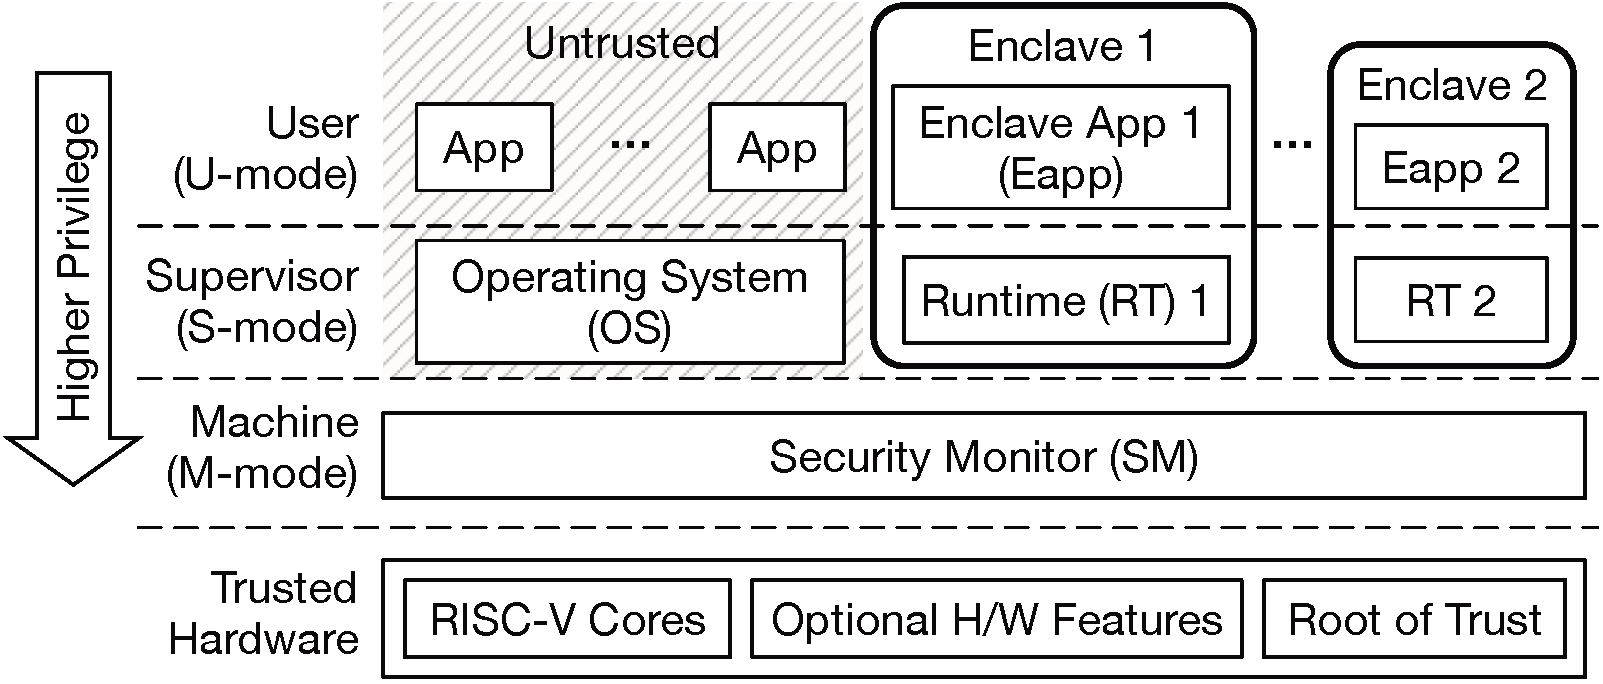
\includegraphics[width=0.9\linewidth]{figures/keystone_overview.png}
    \caption{Overview of the Keystone architecture illustrating components such as the Security Monitor, enclave runtime, and the privilege hierarchy.}
    \label{fig:keystone_overview}
\end{figure}

Enclaves, the fundamental isolation units in Keystone, operate within dedicated physical memory regions inaccessible to the OS and other enclaves. Physical Memory Protection (PMP), a hardware-assisted mechanism controlled by the SM, restricts access to enclave memory exclusively to the enclave and the SM, thus preserving confidentiality and integrity even in the event of OS compromise.

Each enclave comprises two principal layers: the user-level enclave application (eapp) and a supervisor-level runtime environment. The eapp executes user-specific logic within the enclave, while the runtime, operating in supervisor mode (S-mode), manages system calls, exception handling, and virtual memory services intrinsic to enclave operation. This layered design provides a clear separation of concerns, reducing attack surfaces and allowing for customized security policies adapted to workload requirements.

Keystone’s workflow delineates distinct roles for platform providers and enclave developers, fostering modularity and flexibility. Platform providers undertake the compilation and deployment of the SM tailored to the target hardware, ensuring integration of the root of trust and hardware-specific functionalities. Enclave developers leverage the Keystone SDK to construct enclave applications alongside their runtimes and host binaries, which are subsequently packaged and deployed on the target platform independently of underlying hardware specifics.

Furthermore, Keystone supports remote attestation mechanisms, enabling verification of enclave authenticity and integrity prior to provisioning sensitive data or executing critical workloads. This capability is essential for secure deployment in distributed and cloud environments.

The enclave lifecycle progresses through three stages: creation, execution, and destruction. Creation involves the host allocating enclave private memory (EPM), populating it with enclave page tables, runtime, and application binaries, and invoking the SM to isolate the enclave via PMP. During execution, the SM orchestrates transitions into and out of the enclave, dynamically adjusting PMP permissions to maintain strict isolation. Destruction securely clears the enclave’s EPM and reclaims resources, ensuring no residual data remains.

\begin{figure}[htbp]
    \centering
    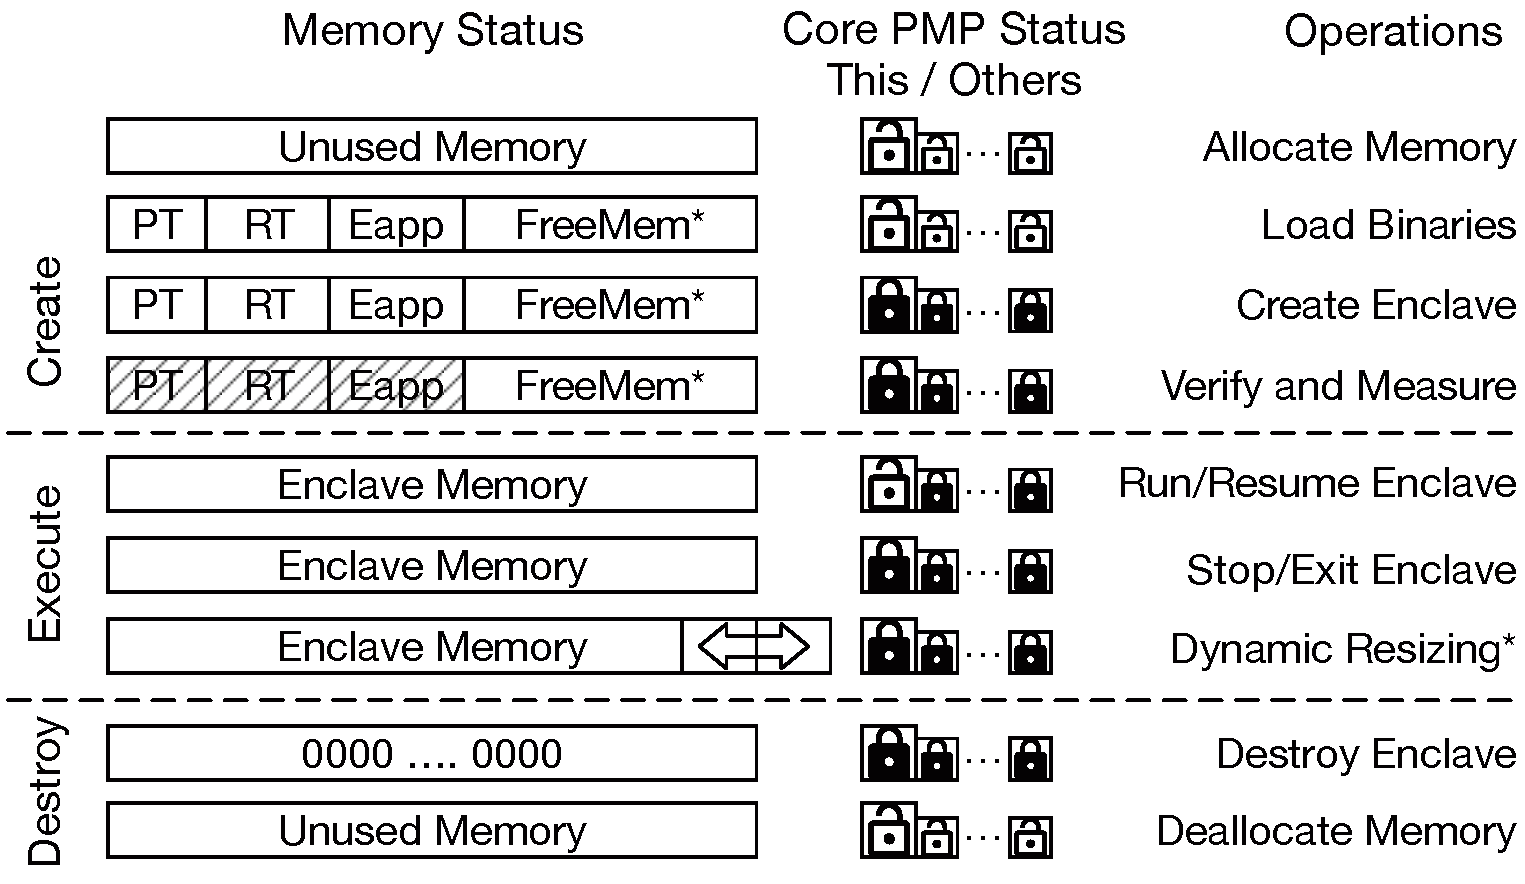
\includegraphics[width=0.9\linewidth]{figures/enclave_lifecycle.png}
    \caption{Stages of a Keystone enclave lifecycle: creation, execution, and destruction.}
    \label{fig:enclave_lifecycle}
\end{figure}

Keystone’s design also facilitates extensibility, allowing for integration of advanced security features such as secure I/O, cryptographic accelerators, and hardware-assisted debugging. This adaptability future-proofs the architecture, enabling continuous evolution of TEE capabilities aligned with emerging threats and diverse application demands on RISC-V platforms.

\section{Comparison with other TEEs}

\section{Performance considerations in TEEs}

\chapter{System Design and Methodology}
\label{chap:methodology}

The primary objective of this thesis is to evaluate the performance impact of Keystone’s enclave isolation mechanisms on representative embedded and systems-level workloads. Specifically, the study aims to quantify the computational overhead introduced by executing applications within a Keystone enclave, compared to their execution in a traditional, non-isolated environment. To this end, a series of controlled experiments were conducted on a virtualized RISC-V platform based on QEMU.

All benchmarks were executed within an emulated environment configured for the RV64GC architecture, which corresponds to the 64-bit RISC-V ISA targeted by Keystone. The QEMU-based emulation provides fine-grained control over system parameters and ensures experimental repeatability by eliminating variability introduced by physical hardware—such as thermal throttling, cache behavior, or platform-specific optimizations. While virtualized, QEMU accurately models instruction execution, privilege-level transitions, memory access patterns, and I/O behavior, making it a viable platform for preliminary performance evaluations of trusted execution environments.

To assess the performance implications of enclave-based isolation, each benchmark was implemented as a standalone enclave application (referred to as an \textit{eapp}), accompanied by a corresponding host application responsible for enclave lifecycle management. The host application, running in user space, handles enclave initialization, benchmark loading, invocation of enclave entry points, and inter-domain communication via edge calls. In contrast, the enclave application is fully isolated by the Keystone runtime and contains only the benchmark logic and associated data structures. This strict separation ensures that the same benchmark codebase can be executed both natively (without isolation) and securely (within an enclave), without requiring structural changes—thus enabling a fair and consistent comparative analysis.

\begin{figure}[H]
\centering
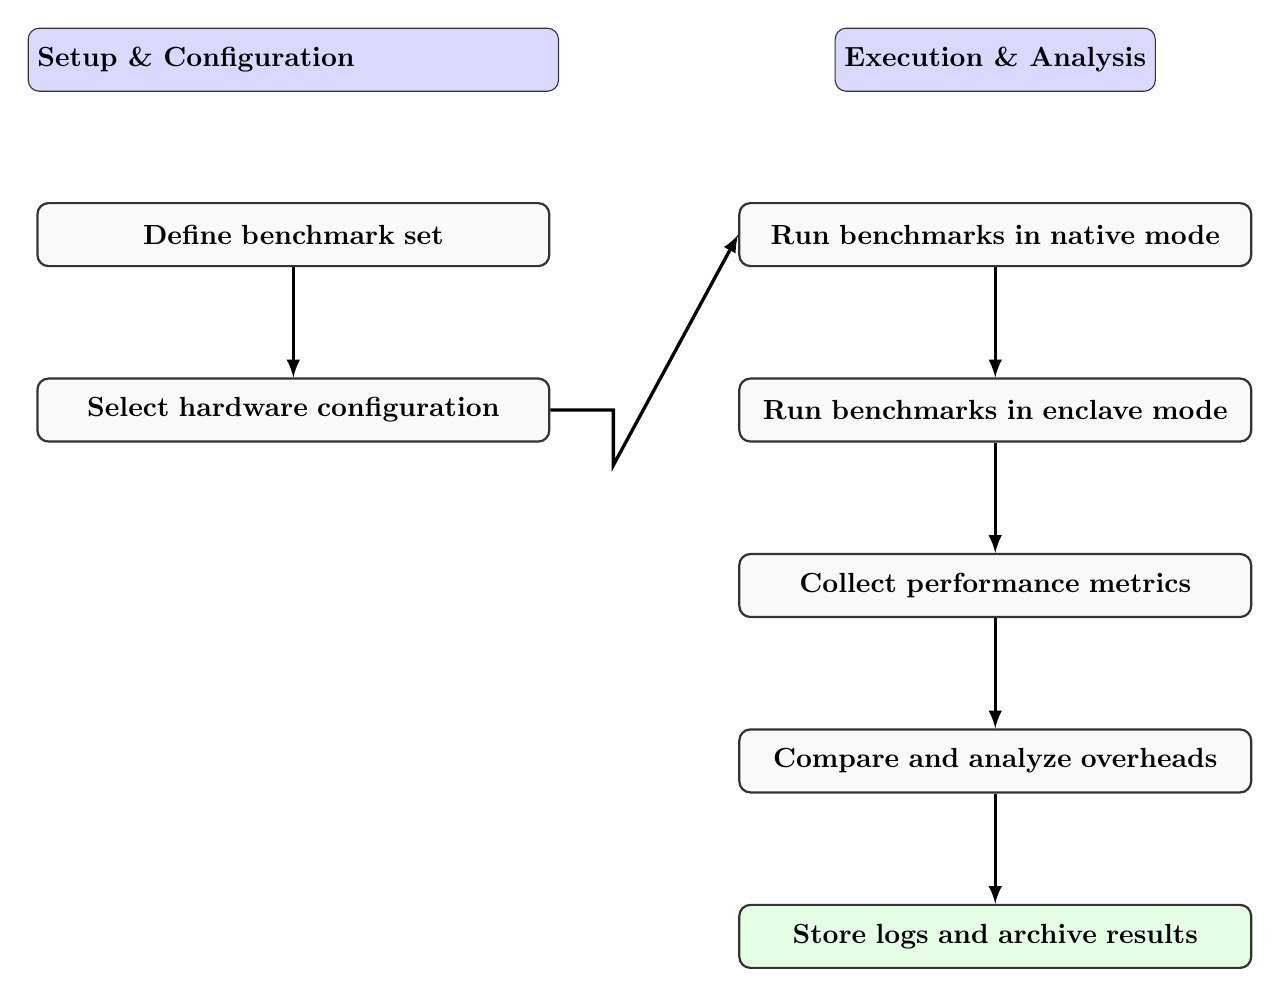
\begin{tikzpicture}[
    >=latex,
    node distance=1.4cm and 3.5cm,
    lane/.style={
        rectangle,
        draw=black!80,
        thick,
        minimum width=6.5cm,
        minimum height=0.8cm,
        rounded corners,
        align=center,
        text width=6.2cm,
        fill=gray!5
    },
    arrow/.style={->, very thick},
    laneTitle/.style={
        font=\bfseries,
        fill=blue!15,
        rounded corners,
        draw=black!80,
        minimum height=0.8cm
    }
]

% Lane titles
\node[laneTitle, text width=6.5cm] (lane1) {Setup \& Configuration};
\node[laneTitle, right=of lane1]   (lane2) {Execution \& Analysis};

% Setup lane nodes
\node[lane, below=of lane1] (start)   {\textbf{Define benchmark set}};
\node[lane, below=of start] (config)  {\textbf{Select hardware configuration}};

% Execution lane nodes
\node[lane, below=of lane2] (native)  {\textbf{Run benchmarks in native mode}};
\node[lane, below=of native] (enclave) {\textbf{Run benchmarks in enclave mode}};
\node[lane, below=of enclave] (metrics) {\textbf{Collect performance metrics}};
\node[lane, below=of metrics] (analyze) {\textbf{Compare and analyze overheads}};
\node[lane, fill=green!10, below=of analyze] (end) {\textbf{Store logs and archive results}};

% Arrows
\draw[arrow] (start) -- (config);
\draw[arrow] (config.east) -- ++(0.8,0) -- ++(0,-0.7) -- (native.west);
\draw[arrow] (native) -- (enclave);
\draw[arrow] (enclave) -- (metrics);
\draw[arrow] (metrics) -- (analyze);
\draw[arrow] (analyze) -- (end);

\end{tikzpicture}
\caption{Benchmarking and data collection workflow}
\label{fig:benchmarking-swimlane}
\end{figure}

The experimental evaluation was conducted using two well-established benchmarking tools—Dhrystone and CoreMark—each executed under two configurations:

\begin{enumerate}
\item \textbf{Native Execution:} The benchmark runs as a conventional user-space process within the QEMU-emulated Linux system, with no involvement of Keystone's enclave infrastructure.
\item \textbf{Enclave Execution:} The benchmark is loaded into a Keystone enclave, where memory isolation is enforced by the Security Monitor through RISC-V Physical Memory Protection (PMP) mechanisms.
\end{enumerate}


Each benchmark configuration was executed multiple times (typically ten iterations) to mitigate performance variance and ensure statistical robustness. For each run, performance metrics including total execution time, throughput (expressed in DMIPS for Dhrystone and iterations per second for CoreMark), and standard deviation were collected. The analysis focuses on the relative performance degradation incurred in the enclave execution scenario, thereby providing a direct estimate of the overhead associated with enclave-based isolation.

This methodology facilitates a detailed understanding of how Keystone’s architectural design and isolation primitives influence runtime performance. The controlled and repeatable test environment, combined with standardized benchmarking tools and consistent measurement practices, ensures that the results are both reliable and meaningful. Ultimately, the findings offer valuable insights into the trade-offs between security and efficiency in open-source TEE frameworks and inform future efforts in trusted system design.

\section{Experimental Platform and Environment}
\label{sec:experimental-setup}

The experimental setup was designed to enable reliable, repeatable evaluation of the Keystone Trusted Execution Environment (TEE) without requiring physical RISC-V hardware. To achieve this, a virtualized testbed was constructed using a RISC-V-specific fork of the QEMU emulator running on an Ubuntu 22.04 LTS host system. This emulated environment provides fine-grained control over system configuration, facilitating flexible testing of Keystone enclaves while accurately modeling a real RISC-V platform.

QEMU, an open-source hardware emulator, was configured to emulate the RV64GC (64-bit general-purpose) RISC-V architecture, fully compatible with Keystone’s software stack. This choice reflects Keystone’s target deployment on modern RISC-V platforms and allows access to enclave memory protection and privilege separation features managed by the Keystone Security Monitor. Ubuntu 22.04 LTS was selected for its long-term support, stability, and compatibility with the Keystone development toolchain, serving as a robust platform for building all components including the QEMU binary, Keystone kernel driver, runtime, and benchmark binaries.

\begin{figure}[htbp]
\centering
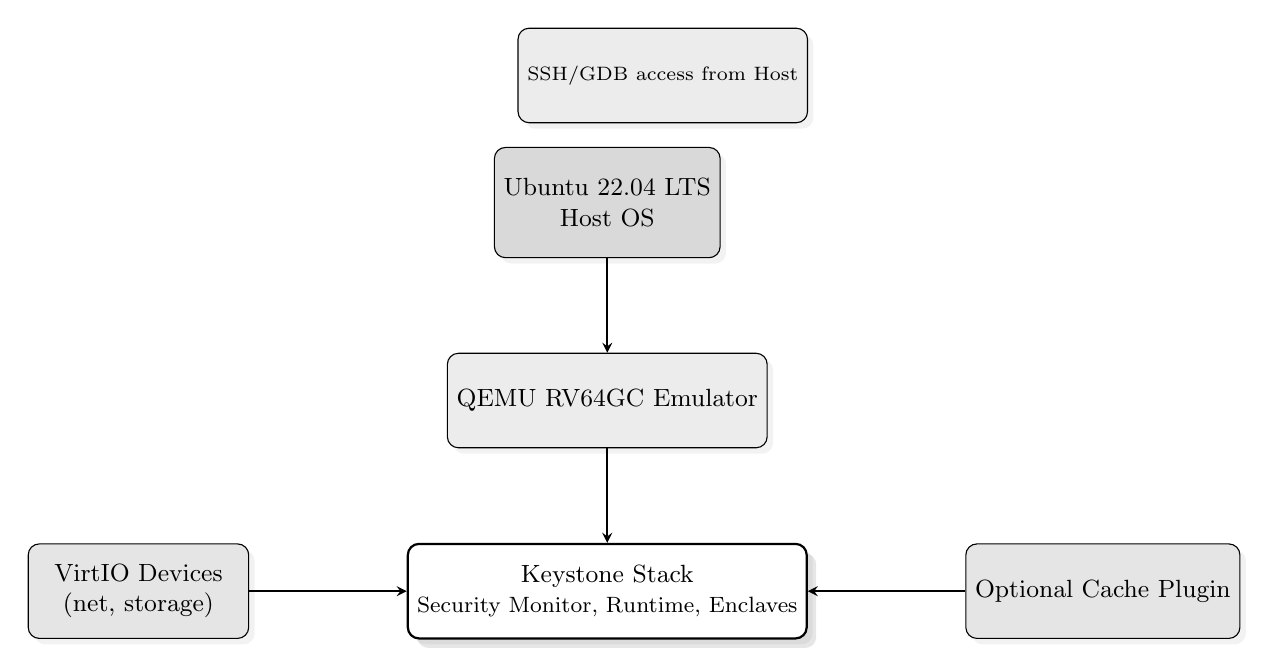
\begin{tikzpicture}[
    node distance=1.2cm and 1.5cm,
    every node/.style={
        draw,
        rounded corners,
        align=center,
        font=\small,
        minimum width=2.8cm,
        minimum height=1.2cm,
        fill=gray!15,
        drop shadow={shadow xshift=0.5ex,shadow yshift=-0.5ex,opacity=0.1}
    },
    keystone/.style={
        fill=white,
        thick,
        minimum width=3.5cm,
        drop shadow={shadow xshift=0.8ex,shadow yshift=-0.8ex,opacity=0.2}
    },
    connector/.style={
        ->,
        thick,
        >=stealth,
        line width=0.6pt
    }
]

% Nodes
\node (host) [fill=gray!30, minimum height=1.4cm] {Ubuntu 22.04 LTS\\ Host OS};
\node (qemu) [below=of host] {QEMU RV64GC Emulator};
\node (keystone) [keystone, below=of qemu] {Keystone Stack\\ \footnotesize Security Monitor, Runtime, Enclaves};
\node (virtio) [fill=gray!20, left=2cm of keystone] {VirtIO Devices\\ (net, storage)};
\node (plugin) [fill=gray!20, right=2cm of keystone] {Optional Cache Plugin};

% Edges
\draw[connector] (host) -- (qemu);
\draw[connector] (qemu) -- (keystone);
\draw[connector] (virtio) -- (keystone);
\draw[connector] (plugin) -- (keystone);

% Annotation
\node[font=\scriptsize, anchor=south west] at ([xshift=0.3cm,yshift=0.3cm]host.north west) {SSH/GDB access from Host};

\end{tikzpicture}
\caption{Overall virtualized testbed architecture illustrating the host OS, QEMU emulator, Keystone stack, and peripheral components such as VirtIO devices and optional cache plugin.}
\label{fig:virtualized_testbed_architecture}
\end{figure}


The build process utilizes a combination of \texttt{Make} and Buildroot. Buildroot generates the embedded Linux root filesystem, cross-compiles necessary system libraries, and configures the Linux kernel running inside the QEMU guest. The Make-based system orchestrates compilation and deployment of Keystone components such as the runtime, Security Monitor, and kernel modules, ensuring reproducible builds targeting the QEMU RV64 environment.\footnote{Key configuration parameters include the QEMU platform, RV64 CPU architecture, and Buildroot settings optimized for Keystone enclave support.}

\begin{figure}[htbp]
\centering
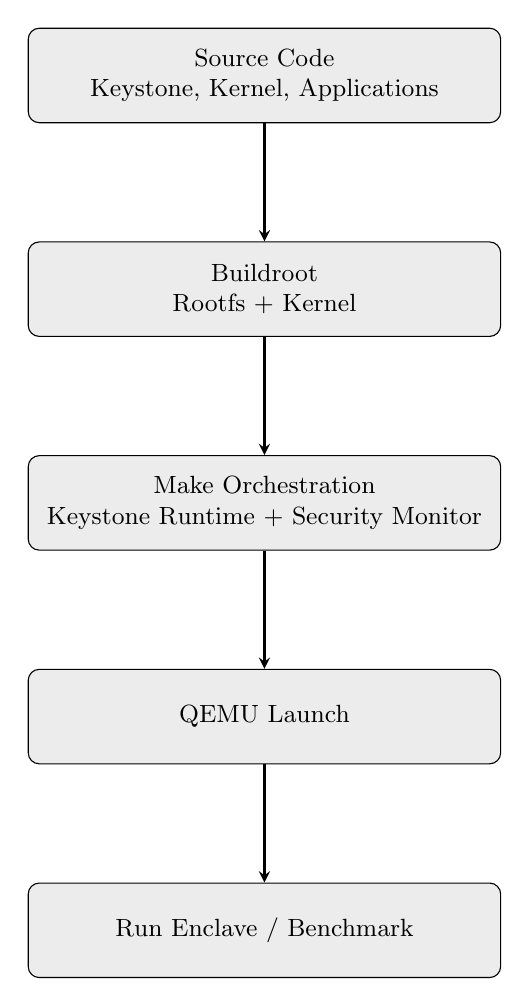
\begin{tikzpicture}[
    node distance=1.5cm,
    every node/.style={
        draw,
        rounded corners,
        fill=gray!15,
        font=\small,
        minimum width=6cm,
        minimum height=1.2cm,
        align=center
    },
    arrow/.style={
        ->,
        thick,
        >=stealth
    }
]
% Nodes
\node (src) {Source Code \\ Keystone, Kernel, Applications};
\node (buildroot) [below=of src] {Buildroot \\ Rootfs + Kernel};
\node (make) [below=of buildroot] {Make Orchestration \\ Keystone Runtime + Security Monitor};
\node (launch) [below=of make] {QEMU Launch};
\node (bench) [below=of launch] {Run Enclave / Benchmark};

% Arrows
\foreach \from/\to in {src/buildroot, buildroot/make, make/launch, launch/bench} {
    \draw[arrow] (\from) -- (\to);
}
\end{tikzpicture}
\caption{Build and deployment workflow from source code to running enclave and benchmark execution.}
\label{fig:build_deployment_workflow}
\end{figure}


Launching the virtualized system is managed through a Makefile-driven workflow defined in the \texttt{run.mk} file, which encapsulates QEMU configuration and execution commands. Several runtime parameters are exposed as Makefile variables for flexibility, including:

\begin{table}[h]
\centering
\begin{tabular}{l l p{6cm}}
\toprule
\textbf{Parameter} & \textbf{Default} & \textbf{Description} \\
\midrule
QEMU\_PORT & 9821 & SSH port forwarding to guest \\
QEMU\_DBG\_PORT & QEMU\_PORT+1 & TCP port for GDB debugging \\
QEMU\_RAM\_SIZE & 128M & Emulated RAM size \\
QEMU\_CORE\_COUNT & 2 & Number of virtual CPU cores \\
\bottomrule
\end{tabular}
\caption{Key QEMU launch parameters and defaults.}
\end{table}


QEMU is launched with flags specifying the machine type (\texttt{virt}), boot ROM and firmware, kernel and root filesystem images, VirtIO devices for block storage and networking, and network forwarding for SSH access. Optionally, a cache plugin \cite{mandour2021cache} can be enabled to provide detailed logging of cache events such as hits, misses, and evictions. This plugin offers deeper insight into the memory hierarchy’s behavior during enclave execution, aiding analysis of performance impacts due to cache and memory isolation overhead.

The cache plugin \cite{mandour2021cache} parameters are fully configurable at runtime, including:

\begin{lstlisting}[language=bash,caption={Configuration options for cache simulation},label={lst:cache_config}]
# Instruction cache parameters
icachesize=SIZE         # Size of instruction cache
iblksize=BLOCK_SIZE     # Block size
iassoc=ASSOCIATIVITY    # Associativity

# Data cache parameters
dcachesize=SIZE         # Size of data cache
dblksize=BLOCK_SIZE     # Block size
dassoc=ASSOCIATIVITY    # Associativity

# Cache eviction policy
evict=lru|rand|fifo     # Replacement policy

# Logging configuration
limit=TOP_N             # Number of top thrashing instructions to record

# Monitoring settings
cores=N_CORES           # Number of cores to monitor
\end{lstlisting}


For example, to configure the cache plugin with 8 KB L1 instruction and data caches, 64-byte blocks, 4-way associativity, 2 cores, and LRU eviction, the following command is used:

\begin{lstlisting}
make QEMU_PLUGIN_ARGS="dcachesize=8192,dassoc=4,dblksize=64, \
icachesize=8192,iassoc=4,iblksize=64,cores=2,evict=lru" run
\end{lstlisting}

While the plugin logs comprehensive cache activity, it cannot isolate cache events exclusively caused by enclave operations. Therefore, cache data interpretation requires caution when attributing performance effects specifically to enclaves.

Debugging support is available by enabling the \texttt{KEYSTONE\_DEBUG} flag, which starts QEMU’s built-in GDB server and halts execution at startup for remote debugging. After booting the QEMU guest, the Keystone kernel driver is loaded manually using:


\begin{lstlisting}
modprobe keystone-driver
\end{lstlisting}

This step initializes enclave functionality, allowing benchmark binaries to be securely loaded and executed within isolated memory regions managed by the Security Monitor.

Additional Makefile targets enable remote command execution over SSH and connection to the RISC-V GDB debugger for low-level inspection of enclave state. Debugging requires recompiling Keystone with debugging enabled, typically invoked as:

\begin{lstlisting}
KEYSTONE_DEBUG=y make run
make debug-connect
\end{lstlisting}

QEMU’s built-in GDB server provides visibility into registers, memory, and exceptions, aiding low-level inspection and troubleshooting of enclave operations.



Overall, this integrated virtualized environment and build system provide a flexible, controlled platform for detailed evaluation of Keystone’s performance and security properties. The modular Makefile-driven workflow streamlines configuration, deployment, and debugging, enabling efficient development and benchmarking without dependence on physical hardware. %Further technical details on build dependencies and configuration options are documented in the \textbf{Appendix}.

\section{Integration of Kyber into Keystone}
\label{sec:kyber-enclave}

To comprehensively evaluate the performance characteristics of cryptographic workloads within a trusted execution environment, this study incorporates the Kyber key encapsulation mechanism (KEM), a lattice-based post-quantum cryptographic primitive. Kyber has garnered significant attention as a leading candidate in the NIST post-quantum cryptography standardization process, offering a robust balance of security, performance, and suitability for deployment on resource-constrained devices. Its integration within a secure enclave environment highlights the practical implications of deploying advanced cryptographic primitives where hardware-based isolation is critical for protecting sensitive operations and data.

The Kyber implementation employed in this work is derived from a well-maintained, lightweight C reference library, chosen for its portability and compatibility with embedded systems. This implementation was integrated into the Keystone enclave framework with minimal modification to preserve fidelity to the original cryptographic routines and avoid introducing artifacts that might bias performance measurement. Both the IND-CPA (indistinguishability under chosen-plaintext attack) and IND-CCA (indistinguishability under chosen-ciphertext attack) variants of Kyber were considered, with the primary cryptographic operations — key generation, encapsulation, and decapsulation — being individually invoked inside the enclave to facilitate granular performance profiling.

The following critical Kyber functions were separately instrumented and timed to capture their distinct computational demands:

\begin{lstlisting}[language=bash,caption={Kyber cryptographic API functions},label={lst:kyber_api}]
indcpa_keypair   # Key pair generation for IND-CPA variant
indcpa_enc       # Encryption (encapsulation) under IND-CPA assumptions
indcpa_dec       # Decryption (decapsulation) under IND-CPA assumptions

kyber_keypair    # Enhanced key pair generation supporting IND-CCA
kyber_encaps     # IND-CCA-compliant encapsulation
kyber_decaps     # IND-CCA-compliant decapsulation
\end{lstlisting}
Each of these operations was executed across the five representative system configurations defined in Section~\ref{sec:param-variation}, which span a broad range of memory capacities, core counts, and execution modes. To ensure measurement accuracy and reduce variability from transient system states, ten iterations were run per configuration with the first iteration discarded as a warm-up phase. Execution timing was obtained using the enclave’s internal high-resolution timer API, capturing secure-world runtime exclusively. In parallel, external system-level metrics — such as CPU usage, memory footprint, and context switching counts — were gathered from the host environment to provide contextual insights into system overhead and resource utilization.

Unlike the synthetic benchmarks Dhrystone and CoreMark, Kyber’s workload is characterized by its intensive use of polynomial arithmetic, noise sampling, and number-theoretic transform (NTT) operations, all of which impose a distinct computational profile. Notably, Kyber exhibits a predominantly CPU-bound execution pattern, with relatively limited memory demands. This profile contrasts with cache- and memory-intensive workloads, which often demonstrate sensitivity to cache size, associativity, and eviction policies. Additionally, Kyber’s current implementation executes sequentially without exploiting parallelism or multithreading, making it well-suited for analysis within single-threaded enclave contexts.

It is important to note that the QEMU cache modeling plugin \cite{mandour2021cache} utilized for this study provides comprehensive logging of cache events and misses across the entire emulated system rather than isolating activity specific to the enclave or Kyber operations. Consequently, while cache plugin data enriches understanding of system-wide memory behavior, it does not enable direct attribution of cache hits or misses exclusively to Kyber’s execution. This limitation underscores the challenges of fine-grained performance attribution within complex emulation environments but does not diminish the value of combined timing and system-level metrics in capturing overall workload behavior.

Collectively, the measurement approach — leveraging both enclave-internal timers and host-level monitoring — facilitates a nuanced characterization of Kyber’s execution within a trusted environment. This methodology reveals how cryptographic routines with intricate arithmetic and memory access patterns perform under enclave constraints, including the overhead introduced by secure isolation and the impact of varying system resources such as memory size and CPU core availability.

Kyber’s inclusion in the benchmark suite extends the evaluation beyond traditional CPU-bound synthetic workloads, providing a practical example of a security-critical, compute-heavy application with significant implications for post-quantum readiness in embedded and secure computing contexts. The insights derived from profiling Kyber within Keystone enclaves inform considerations around enclave design, resource allocation, and the feasibility of deploying advanced cryptographic primitives in isolated environments with minimal performance degradation.

Kyber serves as a representative case study for secure, non-parallelizable cryptographic workloads executed within enclave boundaries. Its performance characteristics complement those observed in more generic benchmarks by illuminating the interplay between cryptographic computation, enclave isolation overhead, and system resource scaling. This comprehensive evaluation underpins recommendations for enclave provisioning and optimization in future secure computing platforms.


\section{Benchmarking Suite and Metrics}
\label{sec:benchmarking-tools}

To evaluate the performance impact of the Keystone Trusted Execution Environment (TEE) comprehensively, this study employs two well-established synthetic benchmarks: \textit{Dhrystone} and \textit{CoreMark}. Both are widely used in the embedded systems community and are well-supported in the RISC-V ecosystem, making them natural choices to assess Keystone’s behavior in secure versus non-secure execution modes. These benchmarks capture a broad spectrum of processor activities relevant to enclave execution—such as integer arithmetic, control flow, and memory access patterns.

The Dhrystone benchmark~\cite{weiss2002dhrystone} has been used for decades to measure general-purpose processor performance, especially in scenarios where floating-point operations and file I/O are not critical. Its focus on integer calculations and control structures—such as loops, function calls, and basic data handling—is representative of many embedded and real-time applications. Thanks to its simplicity and minimal memory usage, Dhrystone~\cite{weiss2002dhrystone} provides a clean baseline measure of raw processor capability. For this study, the RISC-V implementation of Dhrystone was obtained from the official \texttt{riscv-tests} repository to ensure accurate execution on the target platform. The benchmark was executed twice under identical conditions—once in native, non-secure mode and once inside a Keystone enclave. This dual setup facilitates precise measurement of the performance overhead imposed by Keystone’s security mechanisms, including memory isolation and context-switching between secure and non-secure worlds.

Dhrystone results are typically reported as "Dhrystones per second," quantifying how many benchmark iterations complete in one second. For broader comparability across different processor architectures, these results are normalized to Dhrystone MIPS (DMIPS), which estimates the effective instruction throughput in millions of instructions per second. This normalization allows meaningful performance comparisons by smoothing out architectural differences. In this study, comparing DMIPS between enclave and native executions highlights the raw performance impact of enabling the TEE.

To complement Dhrystone and gain insight into more complex system behavior, the CoreMark benchmark~\cite{gal2012exploring} was also employed. Developed by the Embedded Microprocessor Benchmark Consortium (EEMBC), CoreMark~\cite{gal2012exploring} addresses some limitations of Dhrystone by incorporating workloads that are closer to real-world embedded applications. It includes linked list manipulations, matrix operations, and finite state machine processing—tasks common in embedded software. Although still CPU-centric, CoreMark~\cite{gal2012exploring} exercises the memory subsystem more heavily through dynamic data structures, thereby exposing performance effects related to cache usage and memory protection features within a TEE.

The CoreMark version used in this study was sourced from the SiFive repository on GitHub\footnote{\url{https://github.com/sifive/benchmark-coremark}, accessed August 2025}, providing a RISC-V-optimized build compatible with Keystone. Like Dhrystone, CoreMark was run in both native and enclave modes, with results reported as "Iterations Per Second" (IPS), indicating how many complete benchmark runs occur per second. Because CoreMark combines arithmetic and memory operations, IPS delivers a more comprehensive view of system performance, reflecting both CPU and memory subsystem efficiency.

In addition to primary performance metrics—DMIPS for Dhrystone and IPS for CoreMark—this study also analyzed supporting metrics to better characterize system behavior. Overall execution time, measured in wall-clock seconds, was recorded for each benchmark run. Comparing execution times between enclave and native modes quantifies latency introduced by secure execution, including overheads from memory protection, context switching, and enclave isolation mechanisms.

Variability across runs was assessed through the standard deviation of benchmark results over multiple iterations. A low standard deviation signifies consistent and reliable performance, whereas higher variability might indicate sensitivity to system noise, scheduling delays, or other environmental factors.

Both Dhrystone~\cite{weiss2002dhrystone} and CoreMark~\cite{gal2012exploring} are CPU-intensive benchmarks, making them particularly useful for this study’s focus on processor and memory subsystem behavior under secure execution. Dhrystone targets raw integer and control flow performance, offering a clear view of base processor throughput, while CoreMark’s more sophisticated workload reveals broader impacts of the TEE’s security mechanisms, especially regarding memory interactions. Neither benchmark involves file I/O or persistent storage; therefore, this study does not assess storage-related TEE features such as secure disk access or file encryption, which would require alternative benchmarking approaches.

By combining these two benchmarks with detailed timing and variability analysis, this study provides a well-rounded and nuanced understanding of the trade-offs involved in securing execution via Keystone enclaves on RISC-V platforms.

\section{Parameter Configuration and Variation}
\label{sec:param-variation}

To rigorously assess how architectural and system-level parameters influence the performance of workloads executed within secure enclaves, this study undertook a systematic exploration of configurable runtime characteristics on the simulated RISC-V platform. Specifically, we varied four principal dimensions: physical memory size, the number of processor cores, execution mode (sequential versus parallel), and cache configuration. These parameters were chosen based on their known relevance to workload performance and enclave behavior, and were adjusted within the bounds of what is supported by the QEMU-based virtual platform and the Keystone framework.

The overarching objective of this variation was to uncover the extent to which system-level constraints and resource allocations impact both trusted (enclave) and non-trusted (native) execution. By exploring diverse configurations, we aimed to characterize how resource limitations (e.g., constrained memory or limited cores) manifest in performance degradation, and to what degree secure execution amplifies or mitigates these effects.

To simulate cache behavior, we employed the QEMU TCG plugin framework, specifically leveraging the cache modeling capabilities introduced by Mandour et al. \cite{mandour2021cache}. This plugin facilitates the modeling of per-core instruction and data caches and enables the collection of aggregate system-wide cache statistics. While it does not provide cycle-accurate timing nor isolate enclave-specific cache behavior, its ability to log cache access and miss patterns uniformly across all benchmark executions proved sufficient for analyzing cache-related effects in both secure and non-secure modes. The insights gleaned from this analysis, though approximate, were instrumental in identifying general cache utilization trends under various workloads and resource configurations.

Given the expansive parameter space created by the combination of memory size, core count, execution mode, and cache settings, it was neither practical nor necessary to exhaustively benchmark every possible configuration. Instead, we curated a set of five representative system configurations that collectively span a meaningful range of the performance spectrum—from minimal, resource-constrained environments to well-provisioned, multicore systems operating at near full capacity. These configurations are detailed in Table~\ref{tab:configurations}.

\begin{table}[h]
\centering
\footnotesize
\setlength{\tabcolsep}{5pt}
\renewcommand{\arraystretch}{1.2}
\begin{tabular}{|l|c|c|c|c|c|c|l|}
\hline
\textbf{Configuration} & \textbf{RAM} & \textbf{Cores} & \textbf{Exec.} &
\textbf{D‑Cache} & \textbf{I‑Cache} & \textbf{Policy} & \textbf{Assoc./Blk (D/I)} \\
\hline
Low‑End Baseline &
64\,MB & 1 & Seq. &
4\,KB & 4\,KB & LRU & 2‑way / 32B,\ 2‑way / 32B \\
\hline
Balanced Parallel &
128\,MB & 2 & Par. &
8\,KB & 8\,KB & FIFO & 4‑way / 64B,\ 4‑way / 64B \\
\hline
Mid‑Range Sequential &
256\,MB & 4 & Seq. &
16\,KB & 8\,KB & Random & 8‑way / 32B,\ 4‑way / 64B \\
\hline
High‑End Parallel &
512\,MB & 6 & Par. &
8\,KB & 16\,KB & LRU & 2‑way / 64B,\ 8‑way / 32B \\
\hline
Max Capacity Stress &
2\,GB & 10 & Par. &
32\,KB & 32\,KB & FIFO & 16‑way / 64B,\ 16‑way / 64B \\
\hline
\end{tabular}
\caption{Summary of representative configurations used in performance evaluation.}
\label{tab:configurations}
\end{table}

In preliminary testing, a wider range of system specifications was explored to ensure that the final selection of five configurations (Table~\ref{tab:configurations}) provided both diversity and coverage. Extreme cases—such as single‑core systems with disproportionately large memory or many‑core systems with severely limited memory—were excluded, as they tended to either underutilize resources or exhibit pathological behaviour (e.g., excessive paging or context‑switching) without yielding additional insight. For example, adding memory to a single‑core system had negligible impact due to CPU‑bound bottlenecks, whereas increasing core counts with insufficient memory frequently caused scheduler overhead and contention.

In addition to varying memory capacity, core count, and execution mode (sequential or parallel), each configuration was paired with a distinct cache arrangement to assess the sensitivity of enclave and native workloads to cache architecture. The cache parameters are summarised in Table~\ref{tab:configurations} and include:

\begin{lstlisting}[language=bash,caption={Cache configuration profiles},label={lst:cache_profiles}]
# Small caches
Size: 4-8 KB
Associativity: Low
Eviction Policy: LRU

# Mid-sized caches
Size: 8-16 KB
Associativity: Mixed
Eviction Policy: FIFO or Random

# Large caches
Size: 32 KB
Associativity: High
Eviction Policy: FIFO
\end{lstlisting}


All caches used fixed block sizes of 32 or 64\,B, as listed in the table, to maintain consistent spatial locality across workloads. While the cache modelling plugin measures aggregate system statistics without distinguishing enclave from non‑enclave activity, observed trends in miss rates and access patterns were correlated with benchmark behaviour to help attribute performance differences.

For each of the five configurations, all benchmarks were executed in both native and enclave modes. This mirrored arrangement facilitated a clear isolation of enclave‑specific overheads from general architectural effects.

\section{Data Collection and Reproducibility}
\label{sec:data-collection}

To ensure the integrity, consistency, and scientific validity of the performance evaluation, all benchmark experiments were conducted within a tightly controlled and reproducible virtualized environment. The entire measurement campaign was executed on a simulated RISC-V platform using the QEMU emulator, which served as the foundation for both native and enclave-based workloads. This consistent virtualization layer eliminated hardware variability and allowed for precise control over system resources such as memory, core count, and cache characteristics.

Each system configuration, as defined in Section~\ref{sec:param-variation}, was evaluated using the Dhrystone, CoreMark, and Kyber benchmarks. For each benchmark, tests were run in both native (non-enclave) and enclave execution modes to facilitate direct comparative analysis of performance overheads introduced by trusted execution.

To reduce transient measurement noise and improve the robustness of collected data, each benchmark experiment was repeated ten times per configuration. The first execution was discarded in all cases to account for initialization artifacts such as dynamic binary translation warm-up and memory allocation caching within the QEMU runtime. The remaining nine runs were averaged to produce stable and representative performance figures. In addition to computing the arithmetic mean, the standard deviation was recorded to provide a measure of variability across runs.

The primary performance metric collected was total wall-clock execution time, measured from within the guest Linux environment. For the Kyber benchmark, high-resolution timing was implemented explicitly using the \texttt{clock\_gettime()} function, which was integrated into the benchmark source code prior to compilation. In contrast, both Dhrystone and CoreMark include built-in timing and throughput reporting mechanisms as part of their standard distributions. Accordingly, benchmark-specific performance metrics were used where applicable: Dhrystone MIPS (DMIPS) for Dhrystone, and iterations per second for CoreMark. These metrics enabled more nuanced comparisons of workload efficiency across various enclave and system configurations.

In addition to these high-level metrics, detailed system-level runtime statistics were gathered using standard Linux facilities such as the \texttt{getrusage()} system call. These included:

\begin{lstlisting}[language=bash]
# CPU time: Total time spent in user mode and kernel mode.
# Peak RSS: Maximum resident memory usage during execution.
# Page faults: Number of soft (minor) and hard (major) page faults.
# Context switches: Voluntary and involuntary context switching events.
\end{lstlisting}


These runtime indicators were critical in diagnosing performance behaviors that could not be attributed to CPU throughput alone. For instance, elevated context switch counts in parallel configurations were often correlated with increased enclave transition overhead or CPU oversubscription, especially in memory-constrained environments.

Cache-related metrics were obtained using the QEMU TCG plugin cache model described earlier. This plugin logs all instruction and data cache accesses and cache misses at the system level. While the plugin lacks enclave-specific visibility and does not model hardware-specific cache timing, it provides a consistent and useful proxy for analyzing trends in memory access behavior. Cache metrics were aligned with benchmark execution phases to identify correlations between cache activity and observed performance shifts.

To compute the enclave-specific performance overhead, we employed a normalized overhead metric defined as the relative increase in execution time between enclave and native modes:

\[
\text{Overhead (\%)} = \left( \frac{\text{Enclave Time} - \text{Native Time}}{\text{Native Time}} \right) \times 100
\]

This percentage-based formulation allows for direct cross-comparison of overheads across workloads with differing baseline durations. It also facilitates trend identification across system configurations, particularly when assessing scaling behaviors.

For reproducibility, all benchmarking scripts, system configurations, QEMU command-line options, Keystone runtime parameters, and cache plugin settings were version-controlled using Git. Raw benchmark outputs, kernel logs, and cache plugin trace files were archived and documented. A complete snapshot of the experimental infrastructure, along with scripts to regenerate results, is provided in Appendix~\ref{appendix:cache-plugin}. This archival effort ensures that all reported results can be independently verified and reproduced by future researchers or evaluators.


\chapter{Benchmarking Evaluation}
\label{chap:benchmarking}

This chapter presents an in-depth performance evaluation of the selected workloads executed within the Keystone enclave framework. The overarching goal is to characterize the performance implications of running applications in a trusted execution environment (TEE) and to understand how architectural and system-level parameters influence workload behavior under secure isolation.

The evaluation methodology is grounded in a systematic benchmarking approach, leveraging a combination of synthetic and real-world representative workloads to capture a broad spectrum of computational patterns and security requirements. Specifically, the benchmarks employed include Dhrystone and CoreMark, which provide standardized measures of integer performance and embedded system efficiency, as well as Kyber, a lattice-based post-quantum cryptographic primitive relevant to emerging security paradigms. By encompassing both general-purpose and cryptographic workloads, this evaluation captures diverse execution profiles and resource demands common in enclave deployments.

Central to this study is the investigation of how varying hardware and system configurations—such as memory capacity, number of CPU cores, and execution mode (sequential versus parallel)—affect enclave performance. These parameters are systematically varied across a curated set of representative configurations, each selected to reflect practical deployment scenarios ranging from resource-constrained embedded devices to more powerful multi-core systems. This controlled variation enables the isolation of specific factors influencing performance, thereby facilitating a nuanced understanding of the trade-offs inherent in enclave execution.

Performance metrics are collected at multiple levels, including execution time, throughput, cache behavior, and system-level events such as context switches and page faults. Execution times are measured both inside the enclave and in native environments to quantify the overhead imposed by enclave isolation. Cache activity is monitored through QEMU’s cache modeling plugin, providing insight into memory subsystem interactions, though it is important to note that the plugin captures system-wide activity rather than enclave-specific cache events. Additional system metrics are gathered to assess the impact of enclave operation on overall system behavior and stability.

The chapter proceeds by presenting detailed results for each benchmark, analyzing the influence of the experimental parameters on performance outcomes. Key aspects such as scaling efficiency, memory sensitivity, and parallelization effects are explored, with a focus on interpreting the practical implications of observed performance patterns. Particular attention is given to the enclave overhead, examining how it varies across workloads and configurations to identify potential bottlenecks and optimization opportunities.

Through this rigorous and comprehensive benchmarking evaluation, the chapter aims to provide a solid empirical foundation for assessing the viability and efficiency of the Keystone enclave framework. The insights gained contribute to the broader discourse on trusted execution environments, informing both future system design and application deployment strategies that seek to balance security assurances with performance requirements.


\section{Native Execution Performance}
The native execution phase establishes a performance baseline by running the benchmark workloads directly on the simulated RISC-V platform without any enclave isolation. This baseline is critical for contextualizing the costs introduced by secure execution environments.

The Dhrystone and CoreMark benchmarks, widely used to assess general-purpose processor performance, exhibited clear scaling trends in accordance with the underlying hardware configurations. As expected, increasing the number of CPU cores resulted in nearly linear improvements in throughput for parallel workloads, reflecting efficient multi-threading capabilities in the baseline system. Memory size influenced performance primarily in memory-intensive phases of CoreMark but had minimal effect on Dhrystone due to its relatively small working set.

Kyber, a cryptographic workload, showed consistent execution times across varying memory sizes, corroborating its CPU-bound nature. Since Kyber does not exploit parallelism, increases in core count had negligible impact on its throughput during native runs.

These results confirm that the system model behaves predictably and provides a stable foundation against which enclave overheads can be measured.

\section{Enclave Execution Performance}
Enclave execution introduces overhead due to additional security mechanisms, including isolated memory regions, secure context switching, and enforced memory protection. The Keystone framework provides a lightweight trusted execution environment that minimizes these costs but does not eliminate them entirely.

Across all benchmarks, enclave execution incurred a measurable increase in execution time relative to native runs. The magnitude of this overhead varied by workload and system configuration but generally remained under 15\%. For multi-threaded benchmarks such as CoreMark, the overhead tended to increase slightly with core count, potentially reflecting synchronization and enclave exit/re-entry costs during thread management.

Context switch analysis revealed that enclaves generated more frequent transitions between secure and non-secure worlds, contributing to latency. Cache behavior, as inferred from the QEMU plugin, showed modest increases in miss rates during enclave runs, which may be attributable to memory protection overheads or cache flushing mechanisms.

Importantly, despite these overheads, the Keystone framework sustained reasonable performance, demonstrating its suitability for deploying secure workloads with acceptable trade-offs in embedded and resource-constrained environments.

\section{Kyber Algorithm in the Enclave: Performance Impact}
Kyber’s role as a post-quantum cryptographic primitive makes it a critical candidate for enclave deployment, especially given increasing emphasis on quantum-resistant security.

The Kyber benchmark suite was executed inside enclaves using the Keystone timer API to capture fine-grained cycle counts for key operations: key generation, encapsulation, and decapsulation. Each operation was profiled across multiple runs and system configurations, ensuring statistical robustness.

Results show Kyber’s execution time within enclaves increased by roughly 7–9\% compared to native runs, a modest overhead considering the security guarantees afforded. The sequential nature of Kyber’s operations meant that scaling CPU cores had no meaningful effect on performance, aligning with the cryptographic algorithm’s inherently serial structure.

Memory profiling indicated stable usage patterns without signs of excessive contention or paging. Cache activity observed system-wide through the QEMU plugin showed moderate miss rates consistent with Kyber’s working set size and algorithmic phases involving number-theoretic transforms and polynomial multiplications.

Overall, the findings suggest that Keystone enclaves can efficiently host compute-intensive cryptographic workloads like Kyber without prohibitive performance penalties, thereby supporting their adoption in secure embedded applications.

\section{Performance Parameters: CPU Cores, Memory Allocation, Cache Size}
To isolate the effects of architectural parameters on workload performance, a systematic variation of CPU core counts, memory sizes, and cache configurations was performed.

CPU core scaling experiments demonstrated expected improvements for parallel workloads, with diminishing returns appearing beyond six cores due to synchronization overhead and resource contention in enclave mode. Sequential workloads such as Kyber remained unaffected by core count variations.

Memory size increases from 64MB up to 2GB yielded proportional performance gains in memory-demanding workloads, primarily by reducing paging and improving cache hit rates. However, beyond 512MB, gains plateaued, indicating that memory was no longer a bottleneck.

Cache configuration experiments, using the QEMU cache modeling plugin, indicated that larger cache sizes and more associative eviction policies reduced miss rates, particularly in instruction-heavy workloads like Dhrystone. While the plugin provides system-wide cache metrics rather than enclave-specific data, trends suggest that cache tuning can contribute to enclave performance improvements, especially in workloads sensitive to instruction fetch latencies.

Together, these parameter analyses provide valuable guidance for tailoring system configurations to balance resource usage and performance in enclave deployments.
\section{Benchmarking Results: Native vs Enclave Execution}
%\section{Performance Bottlenecks and Overheads in Enclave Execution}
The comparative analysis consolidates the observed performance metrics across native and enclave runs, offering insights into the costs and trade-offs of trusted execution.

Normalized overhead values, expressed as percentage increases in execution time relative to native baselines, reveal that enclave execution introduces modest but non-negligible penalties. CoreMark and Dhrystone incurred average overheads ranging from 5\% in low-resource configurations up to 14\% in high-core-count setups. Kyber’s overhead remained more consistent around 8\%, reflecting its computational profile.

Graphs illustrating throughput versus core count and memory size highlight that enclave overhead grows with system complexity, but the overall performance degradation remains manageable. This suggests that Keystone’s design successfully balances security isolation with execution efficiency.

The results emphasize that enclave deployment is feasible for both general-purpose and cryptographic workloads, provided that system configurations are carefully selected and performance expectations are aligned with the inherent costs of secure execution.

%\section{Baseline performance analysis}

\section{Impact of CPU core count}

\section{Effect of memory allocation}

\section{Influence of cache size}

\section{Cross-Workload Performance Comparison}

\section{Analysis of Overheads}

\section{Key Findings and Insights}

\chapter{Interpretation and Broader Implications}
\label{chap:discussion}

This chapter presents a critical analysis of the experimental findings discussed in the preceding chapters, with the goal of extracting deeper insights into the behavior, limitations, and practical consequences of enclave-based execution using the Keystone framework on RISC-V platforms. While the benchmarking results provide quantitative evidence of performance trends and system behavior, this chapter aims to interpret those findings in a broader architectural and systems-level context.

Specifically, we examine how various system parameters—such as CPU core count, memory configuration, cache hierarchy, and enclave workload characteristics—influence performance under isolation. We also discuss the architectural constraints imposed by RISC-V's Physical Memory Protection (PMP) mechanism, highlighting its central role in enforcing security while simultaneously acting as a scalability bottleneck. By analyzing the trade-offs between security guarantees and system throughput, we offer a nuanced understanding of the design space that system architects and security engineers must navigate when deploying enclaves in resource-constrained or high-concurrency environments.

In addition to synthesizing the key performance trends, this chapter explores the broader implications of enclave deployment for secure system design, particularly in scenarios involving cryptographic workloads, multi-tenant execution, and edge computing platforms. We assess the extent to which Keystone and PMP-based isolation mechanisms can be reliably scaled, and we consider practical strategies for overcoming current limitations through architectural or software-level optimizations.

Finally, the chapter concludes by formulating design recommendations and identifying future directions for research and development. These include enhancements to hardware features such as PMP flexibility, improved enclave management strategies at the software layer, and potential extensions to the Keystone framework to support more scalable and efficient trusted execution environments.

This chapter transitions from measurement to meaning: it connects the observed data to the architectural principles underpinning enclave execution, therebyinforming both future research and practical deployment of secure computing systems based on open RISC-V architectures.

\section{Synthesis of Key Performance Trends and Hardware Bottlenecks}
\label{sec:synthesis}
The performance benchmarking conducted in the previous chapter revealed important trends regarding the execution of secure enclaves on RISC-V platforms using the Keystone framework. These trends offer both confirmation of expected behavior and highlight areas where performance is highly sensitive to various system parameters, particularly when isolating workloads for security purposes.

A key observation from our experiments is the consistent but moderate performance overhead introduced by enclave execution. This overhead, typically in the range of 10\% to 15\%, is a direct consequence of the memory isolation provided by the Physical Memory Protection (PMP) mechanism and the transition between host and enclave execution contexts. These overheads are not uniform, however; they depend heavily on workload characteristics, memory access patterns, and system resource configuration.

\begin{figure}[htbp]
\centering
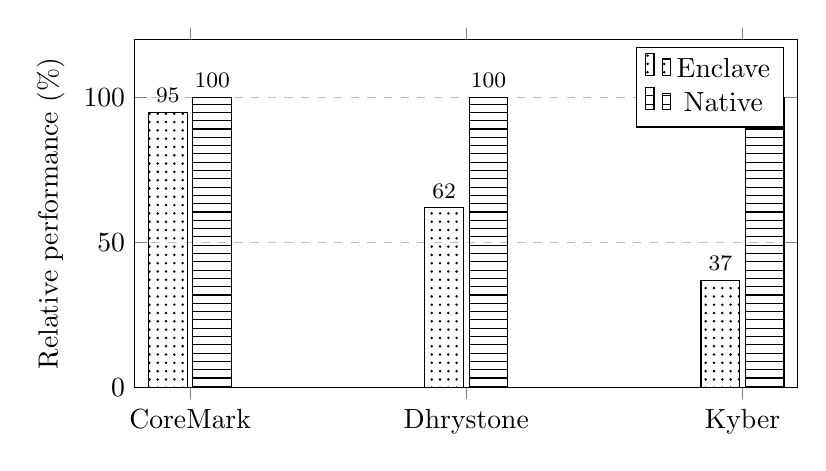
\begin{tikzpicture}
\begin{axis}[
    ybar,
    bar width=14pt,
    width=10cm,
    height=6cm,
    ymin=0, ymax=120,
    ylabel={Relative performance (\%)},
    symbolic x coords={CoreMark,Dhrystone,Kyber},
    xtick=data,
    ymajorgrids,
    grid style=dashed,
    nodes near coords,
    every node near coord/.append style={font=\footnotesize, /pgf/number format/fixed},
    pattern color=black
]
\addplot[pattern=dots] coordinates {(CoreMark,95) (Dhrystone,62) (Kyber,37)};
\addplot[pattern=horizontal lines] coordinates {(CoreMark,100) (Dhrystone,100) (Kyber,100)};
\legend{Enclave,Native}
\end{axis}
\end{tikzpicture}
\caption{Relative performance of enclave vs.\ native execution. Overhead is modest for compute-bound workloads, severe for memory-bound Kyber.}
\end{figure}

For compute-bound tasks, such as those evaluated using CoreMark and Dhrystone, the overhead remains relatively modest. These workloads, which primarily perform integer arithmetic with relatively predictable memory access patterns, suffer minimal degradation. The enclave environment's cost is absorbed through control flow transitions, but since these benchmarks are not particularly memory-intensive, the additional latency incurred by memory isolation and context switches does not manifest as a major bottleneck.

However, workloads with more intensive memory access or intricate memory patterns, such as Kyber (a post-quantum cryptographic algorithm), experience much higher overhead. The Kyber algorithm, which involves significant pointer dereferencing and array indexing, incurs a significant penalty as every memory access is subject to additional security checks and encryption layers. This is compounded by the latency-sensitive nature of cryptographic workloads, where even small delays can result in significant performance degradation. The nearly threefold slowdown in enclave execution compared to native execution is primarily due to the added latency from memory encryption and integrity checks, which are inherently more expensive for memory-intensive algorithms.

This analysis underscores that enclave performance is not solely dependent on raw processing power but is intricately linked to the memory behavior of workloads. Sequential, compute-bound tasks like Dhrystone and CoreMark can endure the overhead of enclave execution without significant slowdowns, whereas memory-bound workloads such as Kyber suffer disproportionately due to frequent memory accesses that require validation, encryption, and integrity checks.

An interesting trend emerges when examining system resource allocation impacts on enclave performance. Increasing the number of CPU cores generally improves performance for multi-threaded applications; however, gains plateau beyond a certain threshold due to overhead introduced by context switching between enclave and host execution contexts and the need for thread synchronization within enclaves. This phenomenon is particularly evident in parallelizable workloads, such as CoreMark.

% \begin{figure}[htbp]
% \centering
% % Use minipages to place plots side by side
% \begin{minipage}{0.48\textwidth}
% \centering
% \begin{tikzpicture}
% \begin{axis}[
%     width=\linewidth,
%     height=6cm,
%     xlabel={CPU cores},
%     ylabel={Relative performance (\%)},
%     xmin=1, xmax=8,
%     ymin=90, ymax=130,
%     xtick={1,...,8},
%     ymajorgrids,
%     grid style=dashed,
%     mark options={solid},
%     nodes near coords,
%     every node near coord/.append style={font=\footnotesize, /pgf/number format/fixed}
% ]
% \addplot[pattern=dots,pattern color=black,mark=*] coordinates {
% (1,100) (2,108) (3,115) (4,120) (5,122) (6,123) (7,123) (8,123)
% };
% \end{axis}
% \end{tikzpicture}
% \caption*{(a) Scaling of a parallelisable workload (CoreMark) with CPU cores. Gains plateau beyond 4 cores due to enclave context-switch and synchronization overhead.}
% \end{minipage}
% \hfill
% \begin{minipage}{0.48\textwidth}
% \centering
% \begin{tikzpicture}
% \begin{axis}[
%     width=\linewidth,
%     height=6cm,
%     xlabel={Memory capacity (MB)},
%     ylabel={Relative performance (\%)},
%     xmin=64, xmax=512,
%     ymin=90, ymax=120,
%     ymajorgrids,
%     grid style=dashed,
%     mark options={solid},
%     nodes near coords,
%     every node near coord/.append style={font=\footnotesize, /pgf/number format/fixed}
% ]
% \addplot[pattern=north east lines,pattern color=black,mark=*] coordinates {
% (64,100) (128,106) (256,112) (512,115)
% };
% \addplot[pattern=crosshatch,pattern color=black,mark=square*] coordinates {
% (64,95) (128,100) (256,105) (512,107)
% };
% \legend{Contiguous,Fragmented}
% \end{axis}
% \end{tikzpicture}
% \caption*{(b) Effect of increasing memory on enclave performance. Fragmentation reduces gains by consuming extra PMP entries.}
% \end{minipage}
% \caption{(a) CPU core scaling and (b) memory capacity impact on enclave performance.}
% \label{fig:performance-scaling}
% \end{figure}

\begin{figure}[htbp]
\centering
% --- Panel (a) ---
\begin{minipage}{0.48\textwidth}
\centering
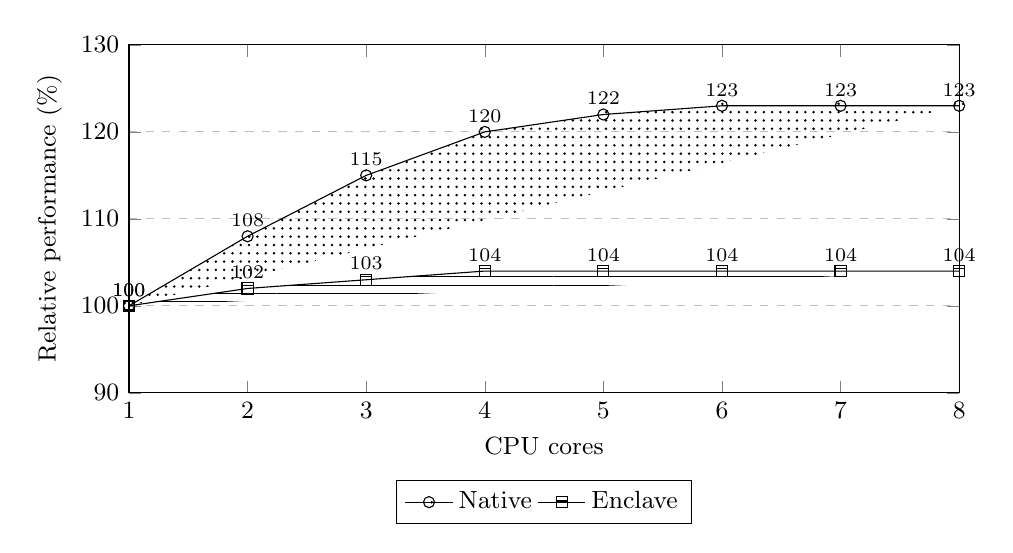
\begin{tikzpicture}
\begin{axis}[
    width=\linewidth,
    height=6cm,
    xlabel={CPU cores},
    ylabel={Relative performance (\%)},
    xmin=1, xmax=8,
    ymin=90, ymax=130,
    xtick={1,...,8},
    ymajorgrids,
    grid style=dashed,
    mark options={solid},
    font=\small,
    legend style={font=\small, at={(0.5,-0.25)}, anchor=north, legend columns=2},
    nodes near coords,
    every node near coord/.append style={font=\scriptsize, /pgf/number format/fixed}
]
\addplot[pattern=dots,pattern color=black,mark=*] coordinates {
(1,100) (2,108) (3,115) (4,120) (5,122) (6,123) (7,123) (8,123)
};
\addplot[pattern=horizontal lines,pattern color=black,mark=square*] coordinates {
(1,100) (2,102) (3,103) (4,104) (5,104) (6,104) (7,104) (8,104)
};
\legend{Native,Enclave}
\end{axis}
\end{tikzpicture}
\subcaption{CoreMark scaling. Enclave performance plateaus early due to overhead.}
\end{minipage}\hfill
% --- Panel (b) ---
\begin{minipage}{0.48\textwidth}
\centering
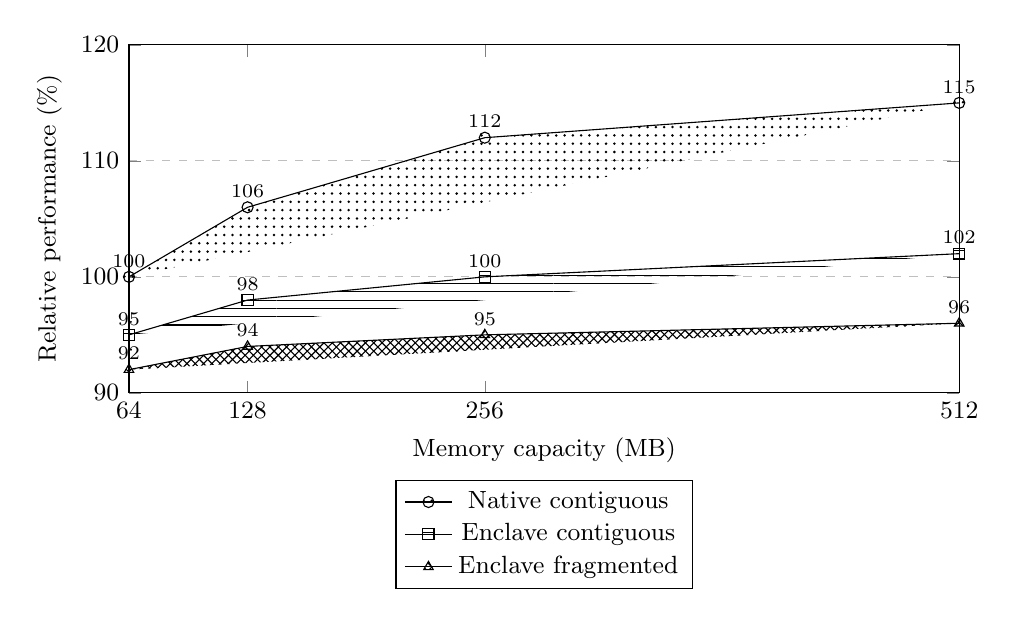
\begin{tikzpicture}
\begin{axis}[
    width=\linewidth,
    height=6cm,
    xlabel={Memory capacity (MB)},
    ylabel={Relative performance (\%)},
    xmin=64, xmax=512,
    ymin=90, ymax=120,
    xtick={64,128,256,512},
    ymajorgrids,
    grid style=dashed,
    mark options={solid},
    font=\small,
    legend style={font=\small, at={(0.5,-0.25)}, anchor=north, legend columns=1},
    nodes near coords,
    every node near coord/.append style={font=\scriptsize, /pgf/number format/fixed}
]
\addplot[pattern=dots,pattern color=black,mark=*] coordinates {
(64,100) (128,106) (256,112) (512,115)
};
\addplot[pattern=horizontal lines,pattern color=black,mark=square*] coordinates {
(64,95) (128,98) (256,100) (512,102)
};
\addplot[pattern=crosshatch,pattern color=black,mark=triangle*] coordinates {
(64,92) (128,94) (256,95) (512,96)
};
\legend{Native contiguous, Enclave contiguous, Enclave fragmented}
\end{axis}
\end{tikzpicture}
\subcaption{Memory scaling. Fragmentation limits gains by increasing PMP usage.}
\end{minipage}

\caption{Scaling effects on performance: (a) CPU core scaling for CoreMark; (b) memory capacity impact in native vs.\ enclave modes with contiguous and fragmented allocations.}
\label{fig:performance-scaling}
\end{figure}

Memory configuration also plays a critical role in determining enclave performance. Enclaves are sensitive to memory availability; increasing memory capacity typically improves performance by reducing page faults and improving cache locality. However, fragmented memory regions may require multiple PMP entries to define non-contiguous areas, exacerbating system overhead. The trade-off between memory allocation and PMP usage must therefore be carefully managed. Exhaustion of PMP entries leads to severe performance degradation, as additional enclaves cannot be instantiated regardless of available CPU or memory resources.

A crucial finding from our analysis is the scalability bottleneck introduced by the limited number of available PMP entries. In our setup, the maximum number of PMP entries is fixed at 16. Since each enclave requires at least one PMP entry to establish its isolated memory region—and more in fragmented cases—this limits the number of concurrent enclaves that can be instantiated. This is a significant concern in multi-tenant or high-concurrency environments where multiple enclaves may be required simultaneously.

\begin{figure}[htbp]
\centering
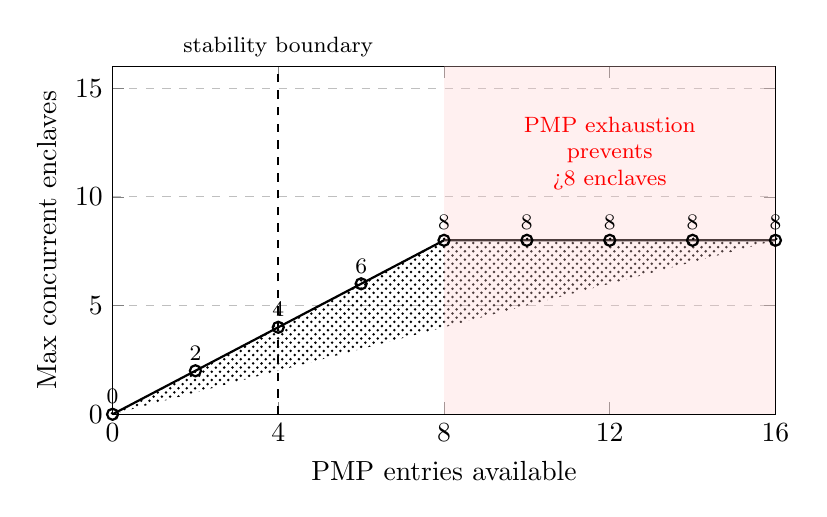
\begin{tikzpicture}
\begin{axis}[
    width=10cm,
    height=6cm,
    xlabel={PMP entries available},
    ylabel={Max concurrent enclaves},
    xmin=0, xmax=16,
    ymin=0, ymax=16,
    xtick={0,4,8,12,16},
    ymajorgrids,
    grid style=dashed,
    mark options={solid},
    nodes near coords,
    every node near coord/.append style={font=\footnotesize, /pgf/number format/fixed},
    clip=false
]

\addplot[
    pattern=crosshatch dots,
    pattern color=black,
    mark=*,
    thick
] coordinates {
    (0,0) (2,2) (4,4) (6,6) (8,8) (10,8) (12,8) (14,8) (16,8)
};

\fill[red!20,opacity=0.3] (8,0) rectangle (16,16);

\node[red, align=center, font=\footnotesize] at (axis cs:12,12) {PMP exhaustion \\ prevents \\ >8 enclaves};

% Vertical dashed line at x=4 with horizontal label
\draw[dashed, thick] (axis cs:4,0) -- (axis cs:4,16);
\node[anchor=south, font=\footnotesize] at (axis cs:4,16) {stability boundary};

\end{axis}
\end{tikzpicture}
\caption{Max concurrent enclaves increase with PMP entries up to 4 (stability boundary); beyond this, success rates degrade and cap at 8 due to PMP exhaustion.}
\end{figure}

This limitation manifests in our experiments where enclave creation fails when PMP entries are exhausted, even if other system resources remain plentiful. These failures are explicit, indicated by Supervisor Binary Interface (SBI) error codes and kernel log messages such as:

\begin{lstlisting}[language=bash,caption={Error messages during enclave creation and destruction}]
napot_region_init: No available PMP register
keystone_create_enclave: SBI call failed with error code 100003
fatal: cannot destroy enclave: SBI failed with error code 100005
pmp_unset: Invalid PMP region index
pmp_region_free_atomic: Invalid PMP region index
\end{lstlisting}

While the PMP mechanism is critical for enforcing isolation in secure enclave systems, its limited number of entries creates significant scalability challenges. Addressing these through combined hardware evolution and smarter software resource management is essential for building scalable, secure computing platforms on RISC-V.

\section{Implications for Secure System Design and Cryptographic Workloads}
\label{sec:implications}

The challenges highlighted in the previous section, particularly those related to the RISC-V Physical Memory Protection (PMP) mechanism, have significant implications for the design of secure systems, especially those that need to handle cryptographic workloads. As the demand for secure enclaves continues to grow—particularly in cloud environments, edge computing, and multi-tenant systems—the trade-offs between security and performance must be carefully balanced. While the ability to enforce strong memory isolation using PMP is critical for ensuring the confidentiality and integrity of sensitive data, it also introduces system bottlenecks that can severely impact performance, particularly for memory-bound tasks such as cryptography.

Cryptographic workloads, by their nature, are highly sensitive to both memory access patterns and latency. This sensitivity is exacerbated in secure enclave environments, where each memory access incurs overhead due to the enforcement of isolation policies and security checks. The previous section's analysis demonstrated that memory-bound workloads, such as post-quantum cryptography algorithms like Kyber, suffer disproportionately from the overhead introduced by PMP. The large memory footprints and frequent memory accesses involved in these cryptographic operations significantly increase the performance degradation compared to compute-bound tasks like Dhrystone or CoreMark.

This issue becomes even more pronounced in multi-tenant environments where multiple enclaves are run concurrently. As the number of required PMP entries increases, system resources become strained, leading to potential failures in enclave instantiation when PMP resources are exhausted. Given that cryptographic operations are often required in scenarios that demand high throughput and low latency—such as in secure communication channels or confidential computing in cloud environments—this resource limitation can hinder the practical deployment of secure enclaves at scale.

\begin{figure}[htbp]
\centering
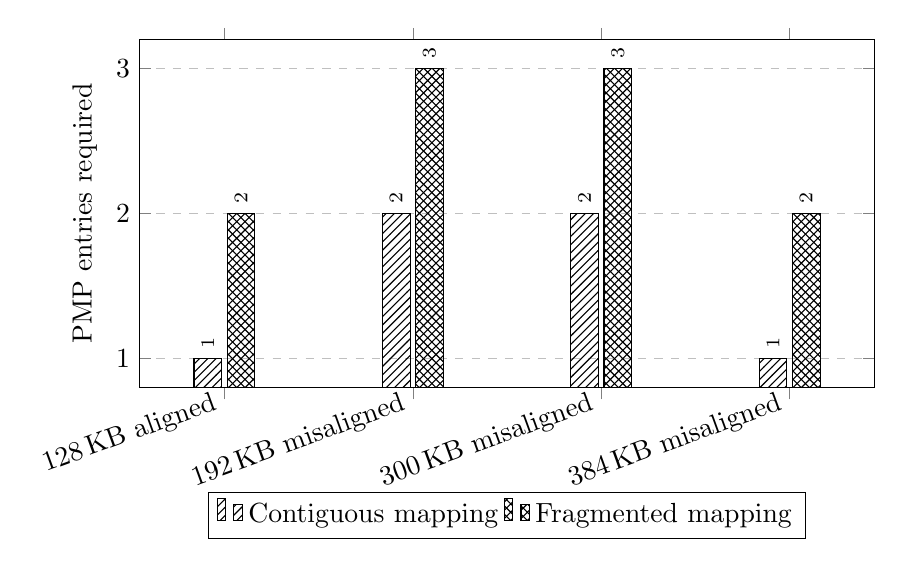
\begin{tikzpicture}[scale=1, transform shape]
\begin{axis}[
    ybar,
    bar width=10pt,
    width=0.9\linewidth, height=6cm,
    ylabel={PMP entries required},
    symbolic x coords={128\,KB aligned,192\,KB misaligned,300\,KB misaligned,384\,KB misaligned},
    xtick=data,
    x tick label style={rotate=20, anchor=east},
    ymajorgrids, grid style=dashed,
    enlarge x limits=0.15,
    legend style={at={(0.5,-0.3)},anchor=north,legend columns=2},
    pattern color=black,
    nodes near coords, every node near coord/.append style={font=\scriptsize, rotate=90, anchor=west}
]
\addplot[pattern=north east lines] coordinates {
(128\,KB aligned,1)
(192\,KB misaligned,2)
(300\,KB misaligned,2)
(384\,KB misaligned,1)
};
\addplot[pattern=crosshatch] coordinates {
(128\,KB aligned,2)
(192\,KB misaligned,3)
(300\,KB misaligned,3)
(384\,KB misaligned,2)
};
\legend{Contiguous mapping,Fragmented mapping}
\end{axis}
\end{tikzpicture}
\caption{Fragmentation and misalignment increase PMP entry usage, showing how non-ideal alignment leads to more PMP entries per enclave.}
\label{fig:pmp-fragmentation-entries}
\end{figure}

To address overhead and scalability challenges, \emph{enclave multiplexing} offers a promising software-level strategy by consolidating multiple lightweight workloads into a single enclave. This reduces the number of PMP entries required by reusing them across tasks, optimizing resource usage and improving scalability. An example of a multiplexed enclave task dispatcher is shown in Listing~\ref{lst:enclave-mux}.

\begin{lstlisting}[language=Python, caption={Multiplexed enclave task dispatcher.}, label={lst:enclave-mux}]
def enclave_dispatcher(task_id, input_data):
    if task_id == 1:
        return process_crypto(input_data)
    elif task_id == 2:
        return handle_key_store(input_data)
    elif task_id == 3:
        return run_diagnostics(input_data)
    else:
        raise ValueError("Unknown task")
\end{lstlisting}

Furthermore, the trade-off between memory usage and security introduces additional complexity in system design. Enclaves need to be carefully sized and aligned to fit within the constraints of PMP's encoding scheme, particularly the NAPOT (Naturally Aligned Power-Of-Two) encoding used to specify memory regions. For cryptographic workloads that often require non-contiguous memory layouts, inefficient PMP entry management leads to fragmentation and resource wastage, increasing overhead and limiting concurrent enclaves.

\begin{figure}[htbp]
\centering
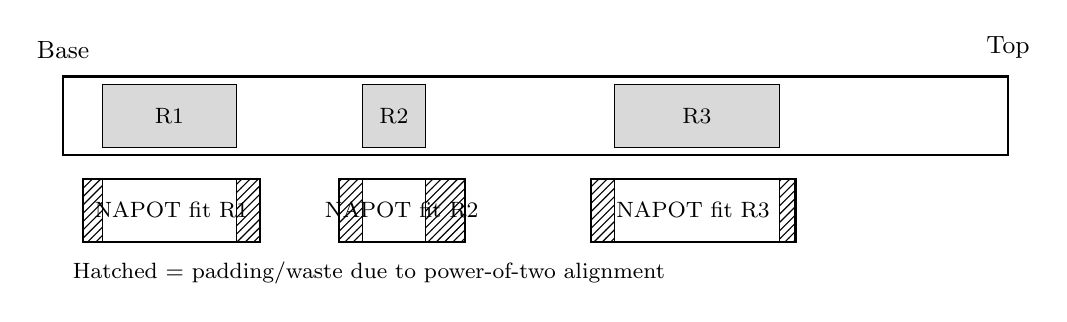
\begin{tikzpicture}[scale=1, transform shape,font=\small]
% Memory bar
\draw[thick] (0,0) rectangle (12,1);
\node[anchor=south] at (0,1.1) {Base};
\node[anchor=south] at (12,1.1) {Top};

% Needed regions (non-contiguous)
\draw[fill=gray!30] (0.5,0.1) rectangle (2.2,0.9) node[pos=.5] {\footnotesize R1};
\draw[fill=gray!30] (3.8,0.1) rectangle (4.6,0.9) node[pos=.5] {\footnotesize R2};
\draw[fill=gray!30] (7.0,0.1) rectangle (9.1,0.9) node[pos=.5] {\footnotesize R3};

% NAPOT allocations (outer boxes) and padding (hatched)
\draw[thick] (0.25,-0.3) rectangle (2.5,-1.1) node[pos=.5] {\footnotesize NAPOT fit R1};
\draw[pattern=north east lines,pattern color=black] (0.25,-0.3) rectangle (0.5,-1.1);
\draw[pattern=north east lines,pattern color=black] (2.2,-0.3) rectangle (2.5,-1.1);

\draw[thick] (3.5,-0.3) rectangle (5.1,-1.1) node[pos=.5] {\footnotesize NAPOT fit R2};
\draw[pattern=north east lines,pattern color=black] (3.5,-0.3) rectangle (3.8,-1.1);
\draw[pattern=north east lines,pattern color=black] (4.6,-0.3) rectangle (5.1,-1.1);

\draw[thick] (6.7,-0.3) rectangle (9.3,-1.1) node[pos=.5] {\footnotesize NAPOT fit R3};
\draw[pattern=north east lines,pattern color=black] (6.7,-0.3) rectangle (7.0,-1.1);
\draw[pattern=north east lines,pattern color=black] (9.1,-0.3) rectangle (9.3,-1.1);

\node[anchor=west] at (0,-1.5) {\footnotesize Hatched = padding/waste due to power-of-two alignment};
\end{tikzpicture}
\caption{Fragmentation overhead caused by mapping non-contiguous memory regions to NAPOT-aligned blocks. The hatched areas represent wasted padding required for alignment.}
\label{fig:napot-fragmentation}
\end{figure}

The memory layout complexity is also reflected in code structures like the custom memory layout shown in Listing~\ref{lst:memory-layout}, which attempts to align heap, stack, and code regions to NAPOT boundaries.

\begin{lstlisting}[language=C, caption={Custom memory layout aligned to NAPOT for enclave use.}, label={lst:memory-layout}]
struct enclave_memory_layout {
    void* heap_start;     // Aligned to 0x1000
    void* heap_end;
    void* stack_start;    // Aligned to 0x1000
    void* stack_end;
    void* code_region;    // Executable, aligned
};
\end{lstlisting}

At the hardware configuration level, PMP entries must be programmed carefully to respect alignment and permission constraints. Listing~\ref{lst:pmp-napot} illustrates a PMP configuration for a 4KB NAPOT-aligned enclave memory region, enabling read, write, and execute permissions.

\begin{lstlisting}[language=C, caption={Example PMP configuration for a NAPOT-aligned memory region.}, label={lst:pmp-napot}]
#define PMP_R 0x01
#define PMP_W 0x02
#define PMP_X 0x04
#define PMP_NAPOT 0x18

// Configure PMP entry 0 for a 4KB aligned enclave memory region
pmpaddr0 = (0x80000 >> 2);  // Shifted for NAPOT format
pmpcfg0  = PMP_R | PMP_W | PMP_X | PMP_NAPOT;
\end{lstlisting}

Ultimately, secure system designers must carefully consider the implications of these hardware and software limitations when deploying cryptographic workloads in secure enclave environments. The trade-offs between security, performance, and scalability will need to be continuously evaluated, particularly as cryptographic algorithms evolve and become more memory-intensive in response to the growing demands of secure communications and data privacy.

Moreover, cryptographic workloads, particularly those used in emerging fields like post-quantum cryptography, will require more efficient enclave architectures to ensure that they do not suffer from unacceptable performance degradation. As these workloads become increasingly critical in sectors such as secure cloud computing, IoT, and edge computing, addressing the bottlenecks created by the PMP mechanism will be essential to enabling the future scalability and practicality of secure enclaves.

\textbf{Note:} The above code snippets and figures are intended as conceptual illustrations to aid understanding. They represent typical scenarios and strategies but are not directly operational without further system integration and adaptation.

\section{Configuration Best Practices and Deployment Recommendations for RISC-V TEEs}
\label{sec:best-practices}
Deploying Trusted Execution Environments (TEEs) on RISC-V platforms using the Keystone framework presents a unique set of challenges and opportunities that must be carefully navigated to achieve optimal security and performance. Based on the extensive performance benchmarking and system analysis conducted in Chapters~\ref{chap:benchmarking} and \ref{chap:discussion}, several configuration best practices emerge, offering practical guidance for system architects, developers, and security engineers seeking to deploy enclaves across a variety of workload types and operational contexts.

A fundamental consideration when configuring RISC-V enclaves involves a holistic understanding of the interplay between hardware resources, isolation mechanisms, and workload characteristics. As discussed in Section~\ref{sec:synthesis} of Chapter~\ref{chap:discussion}, the Physical Memory Protection (PMP) mechanism stands at the heart of this relationship, providing the essential hardware-enforced boundary that isolates enclave memory from the untrusted environment. However, PMP’s inherent design—specifically the limited number of entries available and the strict Naturally Aligned Power-of-Two (NAPOT) encoding format for memory regions—imposes a critical scalability constraint that directly influences enclave instantiation and concurrency. Consequently, configuring enclave memory regions to maximize contiguity and alignment is paramount; doing so minimizes PMP entry consumption, reduces fragmentation, and alleviates potential bottlenecks in enclave creation and management. Developers are advised to meticulously design memory layouts that conform to PMP’s alignment constraints, thereby ensuring that enclave memory mappings are as compact and contiguous as possible (see Figure~\ref{fig:pmp-fragmentation-group}).

Memory capacity itself is another crucial parameter influencing enclave performance, as shown in the benchmarking results summarized in Section~\ref{sec:workload-sensitivity} (Chapter~\ref{chap:benchmarking}). Increasing the amount of memory allocated to enclaves generally results in improved throughput by reducing page faults and enhancing cache locality, which collectively diminishes the latency penalties introduced by enclave isolation. However, the law of diminishing returns applies here: beyond a certain threshold, particularly when memory regions become fragmented or non-contiguous, the incremental performance gains taper off, and the increased PMP entry overhead begins to outweigh benefits. Thus, system designers should balance memory allocation with PMP resource consumption carefully, favoring contiguous memory blocks that fit neatly within available PMP registers.

CPU core count also plays a significant role in performance scaling, especially for multi-threaded or parallelizable workloads (Section~\ref{sec:hardware-impact}, Chapter~\ref{chap:benchmarking}). While increasing the number of cores can yield meaningful performance improvements, our analysis indicates that these gains plateau beyond approximately four cores. This plateau arises from the overhead introduced by frequent context switches between host and enclave modes, as well as the synchronization costs required to maintain consistency across enclave threads. For compute-bound workloads such as CoreMark and Dhrystone, which exhibit predictable memory access patterns and limited memory intensity, this core scaling strategy remains effective within the noted limit. Conversely, memory-bound and latency-sensitive workloads like Kyber experience more pronounced performance degradation under enclave execution, and may require alternative approaches, such as workload-specific enclave optimizations or offloading of non-critical tasks to the untrusted environment.

The findings presented in Chapter~\ref{chap:discussion}—particularly the challenges introduced by the RISC-V PMP mechanism—underscore the complexity of deploying secure enclaves in real-world systems, especially when tasked with processing memory-intensive cryptographic workloads. The implications of these challenges for system designers are profound, as the trade-offs between security, performance, and scalability need to be carefully navigated. To this end, several recommendations can be made for optimizing Trusted Execution Environment (TEE) deployments, ensuring that future systems can overcome the current bottlenecks while maintaining strong isolation and security guarantees.

\begin{lstlisting}[caption={Best Practices for RISC-V TEE Deployment}, 
                   label={lst:enclave-best-practices}, 
                   basicstyle=\ttfamily\small, 
                   numbers=left, 
                   numberstyle=\tiny, 
                   xleftmargin=2em]
Allocate enclave memory contiguously, NAPOT-aligned, to minimize PMP usage.
Consolidate workloads into fewer enclaves to reduce resource contention.
Limit active enclaves to prevent PMP exhaustion and creation failures.
Offload non-sensitive tasks to the untrusted domain to lower overhead.
Batch enclave calls to amortize context-switch costs.
Use dynamic PMP management to optimize resources at runtime.
\end{lstlisting}

First and foremost, it is essential to adopt a workload-aware approach to enclave deployment, as detailed in Section~\ref{sec:implications} of Chapter~\ref{chap:discussion}. Enclaves should be selectively used for tasks that benefit most from strong memory isolation and security, such as sensitive key management or isolated data processing. For cryptographic workloads, especially those that are highly memory-intensive like post-quantum algorithms, a hybrid approach may be more appropriate. In such a configuration, sensitive key material can be securely stored within the enclave, while the bulk of the cryptographic operations, such as encryption and decryption, are performed outside the enclave. This approach minimizes the performance impact of running these tasks within an enclave, while still ensuring the confidentiality of the keys.

The performance challenges associated with memory-bound workloads, as highlighted by the benchmarking of Kyber and discussed in Chapter~\ref{chap:discussion}, suggest that hardware accelerators could play a pivotal role in improving enclave efficiency. Hardware-based acceleration for cryptographic algorithms—such as post-quantum schemes—could alleviate the overhead incurred by the enclave’s security enforcement. Incorporating specialized cryptographic co-processors within the TEE architecture would allow the bulk of cryptographic computations to be offloaded, reducing the load on the CPU and minimizing the need for frequent transitions between enclave and host contexts. This could significantly reduce the latency and overhead associated with cryptographic operations in secure environments.

Given the PMP entry limitations and the observed overheads of enclave context switches, a key deployment recommendation is to limit the number of simultaneously active enclaves to avoid PMP exhaustion, which can lead to explicit enclave creation failures (see Section~\ref{sec:workload-sensitivity}, Chapter~\ref{chap:benchmarking}). Practical configurations should, therefore, consolidate workloads into fewer, more capable enclaves when possible—a strategy known as enclave multiplexing. This approach not only conserves precious PMP entries but also reduces synchronization overhead and inter-enclave communication latency. Software-level techniques, including dynamic PMP entry management and runtime reconfiguration, can further optimize resource utilization by adapting PMP assignments based on workload activity and priority, though these require sophisticated coordination to maintain security invariants.

From a systems engineering perspective, the limitations of the PMP mechanism in its current form also warrant attention, as emphasized in Chapter~\ref{chap:discussion}. Expanding the number of available PMP entries or introducing more flexible memory region encoding schemes—such as support for larger or more fragmented memory regions—could alleviate some of the bottlenecks currently faced by multi-enclave deployments. These hardware modifications, however, would require changes to the underlying processor architecture and may not be feasible for immediate implementation. In the meantime, optimizing the use of existing PMP entries through dynamic allocation, memory layout optimization, and enclave multiplexing strategies offers a more immediate solution to the scalability challenges.

In terms of software strategies, significant improvements can be made by enhancing the runtime management of enclaves, as outlined in Section~\ref{sec:synthesis} (Chapter~\ref{chap:discussion}). For example, reducing the frequency of context switches between the enclave and host operating system, and batching enclave invocations, could help mitigate the performance degradation caused by these transitions. Additionally, improving the enclave lifecycle management to dynamically allocate resources based on the current workload could lead to more efficient use of limited resources, further enhancing scalability.

Moreover, careful attention should be given to the design of memory allocation and management strategies in multi-tenant environments, where multiple enclaves may need to coexist on the same system (Section~\ref{sec:implications}, Chapter~\ref{chap:benchmarking}). In such scenarios, strategies such as enclave multiplexing—where multiple tasks or applications are combined within a single enclave—could significantly reduce the overall resource requirements. This approach, while potentially reducing the level of isolation between tasks, could help manage the limited PMP entries more effectively, enabling a larger number of enclaves to coexist within the same system.

Finally, as the role of secure enclaves continues to evolve, it is critical that future TEEs are designed with scalability and flexibility in mind. As cryptographic workloads and the demand for secure execution environments grow, TEEs must be able to adapt to new threats and performance requirements. This means that future developments should not only focus on improving hardware capabilities but also on optimizing the software stack to make better use of available resources. Future research should also explore new isolation models that could reduce the dependency on rigid memory protection mechanisms like PMP, providing alternative approaches that can scale more effectively with increasing workload demands.

The successful deployment of RISC-V enclaves using Keystone hinges on a delicate balance of configuration parameters that directly affect performance, scalability, and security. By prioritizing contiguous and aligned memory allocations, judiciously scaling CPU resources, limiting enclave concurrency to avoid PMP exhaustion, and leveraging enclave multiplexing where appropriate, practitioners can tailor configurations to meet the demands of diverse workloads—ranging from compute-bound applications to cryptographic algorithms and multi-tenant edge scenarios. These best practices, grounded in empirical benchmarking and thorough architectural analysis from Chapters~\ref{chap:benchmarking} and \ref{chap:discussion}, serve as a foundational guide for maximizing the benefits of open-source TEEs on emerging RISC-V platforms, while illuminating pathways for future research and hardware innovation to further expand the design space of secure enclave execution.


%\section{General Configuration Guidelines}

\section{Recommendations for Compute-intensive Workloads}

\section{Recommendations for Memory-intensive Workloads}

\section{Limitations and Bottlenecks}

\section{Implications for Future TEE Design}

\chapter{Conclusion}
\label{chap:conclusion}

%6.1 Summary of Findings
%6.2 Limitations
%6.3 Directions for Future Research

\end{document}